\chapter{Dane i zmienne}
\label{ch:dane}

Dane odgrywają kluczową rolę w analizie i prognozowaniu cen energii na Rynku Dnia Następnego (RDN) w Polsce, stanowiąc fundament dla modeli uczenia maszynowego zastosowanych w niniejszej pracy. Zbiór danych stworzony w pracy obejmuje okres od 1 stycznia 2016 roku do 31 grudnia 2024 roku i zawiera dane godzinowe. Zbiór danych zawiera różnorodne zmienne, które można podzielić na kilka kategorii, które zostaną opisane w tym dziale. Duża ilość danych pochodzi z \gls{pse} \cite{PSEOLD}, czyli otwartej platformie, która dostarcza różnego rodzaju danych dostępnych dla analizy. Warto zauważyć, że od 14 czerwca 2024 roku PSE zmieniła sposób raportowania danych i przeszła na nową stronę \cite{PSENEW}, w związku z tym PSE posiada dwie oddzielne strony do raportów historycznych przed i po tym dniu. Wiele z danych zostały pobrane również ze strony energy.instrat.pl. Jest to strona, która pobiera dane z platformy PSE i udostępnia je w sposób wygodniejszy, dzięki czemu arkusze csv z dowolnego okresu czasowego z dowolną częstotliwością można pobrać jednym przyciskiem myszy. Dane dotyczące cen paliw kopalnych oraz kursów walut (np. PLN/USD) zostały pozyskane z innych źródeł, takich jak publiczne bazy danych rynkowych i platformy finansowe. Niniejszy rozdział szczegółowo opisuje zmienną zależną i zmienne niezależne, podzielone na kategorie, a także prezentuje kluczowe cechy danych za pomocą tabel i wykresów, co wyjaśnia dobór zmiennych i pozwala na lepsze zrozumienie ich specyfiki i wyzwań związanych z modelowaniem.

\section{Zmienna zależna}
Zmienna zależna w niniejszej pracy to fixing\_i\_price, czyli cena energii elektrycznej na Rynku Dnia Następnego (RDN) w Polsce, wyrażona w PLN/MWh. Dane dotyczące tej zmiennej zostały pobrane z wymienionej platformy energy.instrat.pl w granulacji godzinowej. Zbiór danych obejmuje okres od 1 stycznia 2016 roku do 31 grudnia 2024 roku. Statystyki opisowe zmiennej fixing\_i\_price przedstawiono w Tabeli poniżej. 
\begin{table}[H]
    \centering
    \begin{tabular}{|l|r|}
    \hline
    \textbf{Statystyka} & \textbf{Wartość} \\ \hline
    Średnia             & 344.10 PLN/MWh   \\ \hline
    Odchylenie std.     & 268.35 PLN/MWh   \\ \hline
    Minimum             & -360.00 PLN/MWh  \\ \hline
    25\% (Q1)           & 176.11 PLN/MWh   \\ \hline
    Mediana             & 250.00 PLN/MWh   \\ \hline
    75\% (Q3)           & 434.84 PLN/MWh   \\ \hline
    Maksimum            & 3812.45 PLN/MWh  \\ \hline
    \end{tabular}
    \caption{Podstawowe statystyki zmiennej fixing\_i\_price}
    \label{tab:fixing-i-price-stats}
\end{table}

Aby lepiej zrozumieć dynamikę cen energii na RDN, przeanalizowano ich zmienność w całym okresie badania. Rysunek poniżej przedstawia zmienność cen energii w czasie zebranych danych.

\begin{figure}[H]
    \centering
    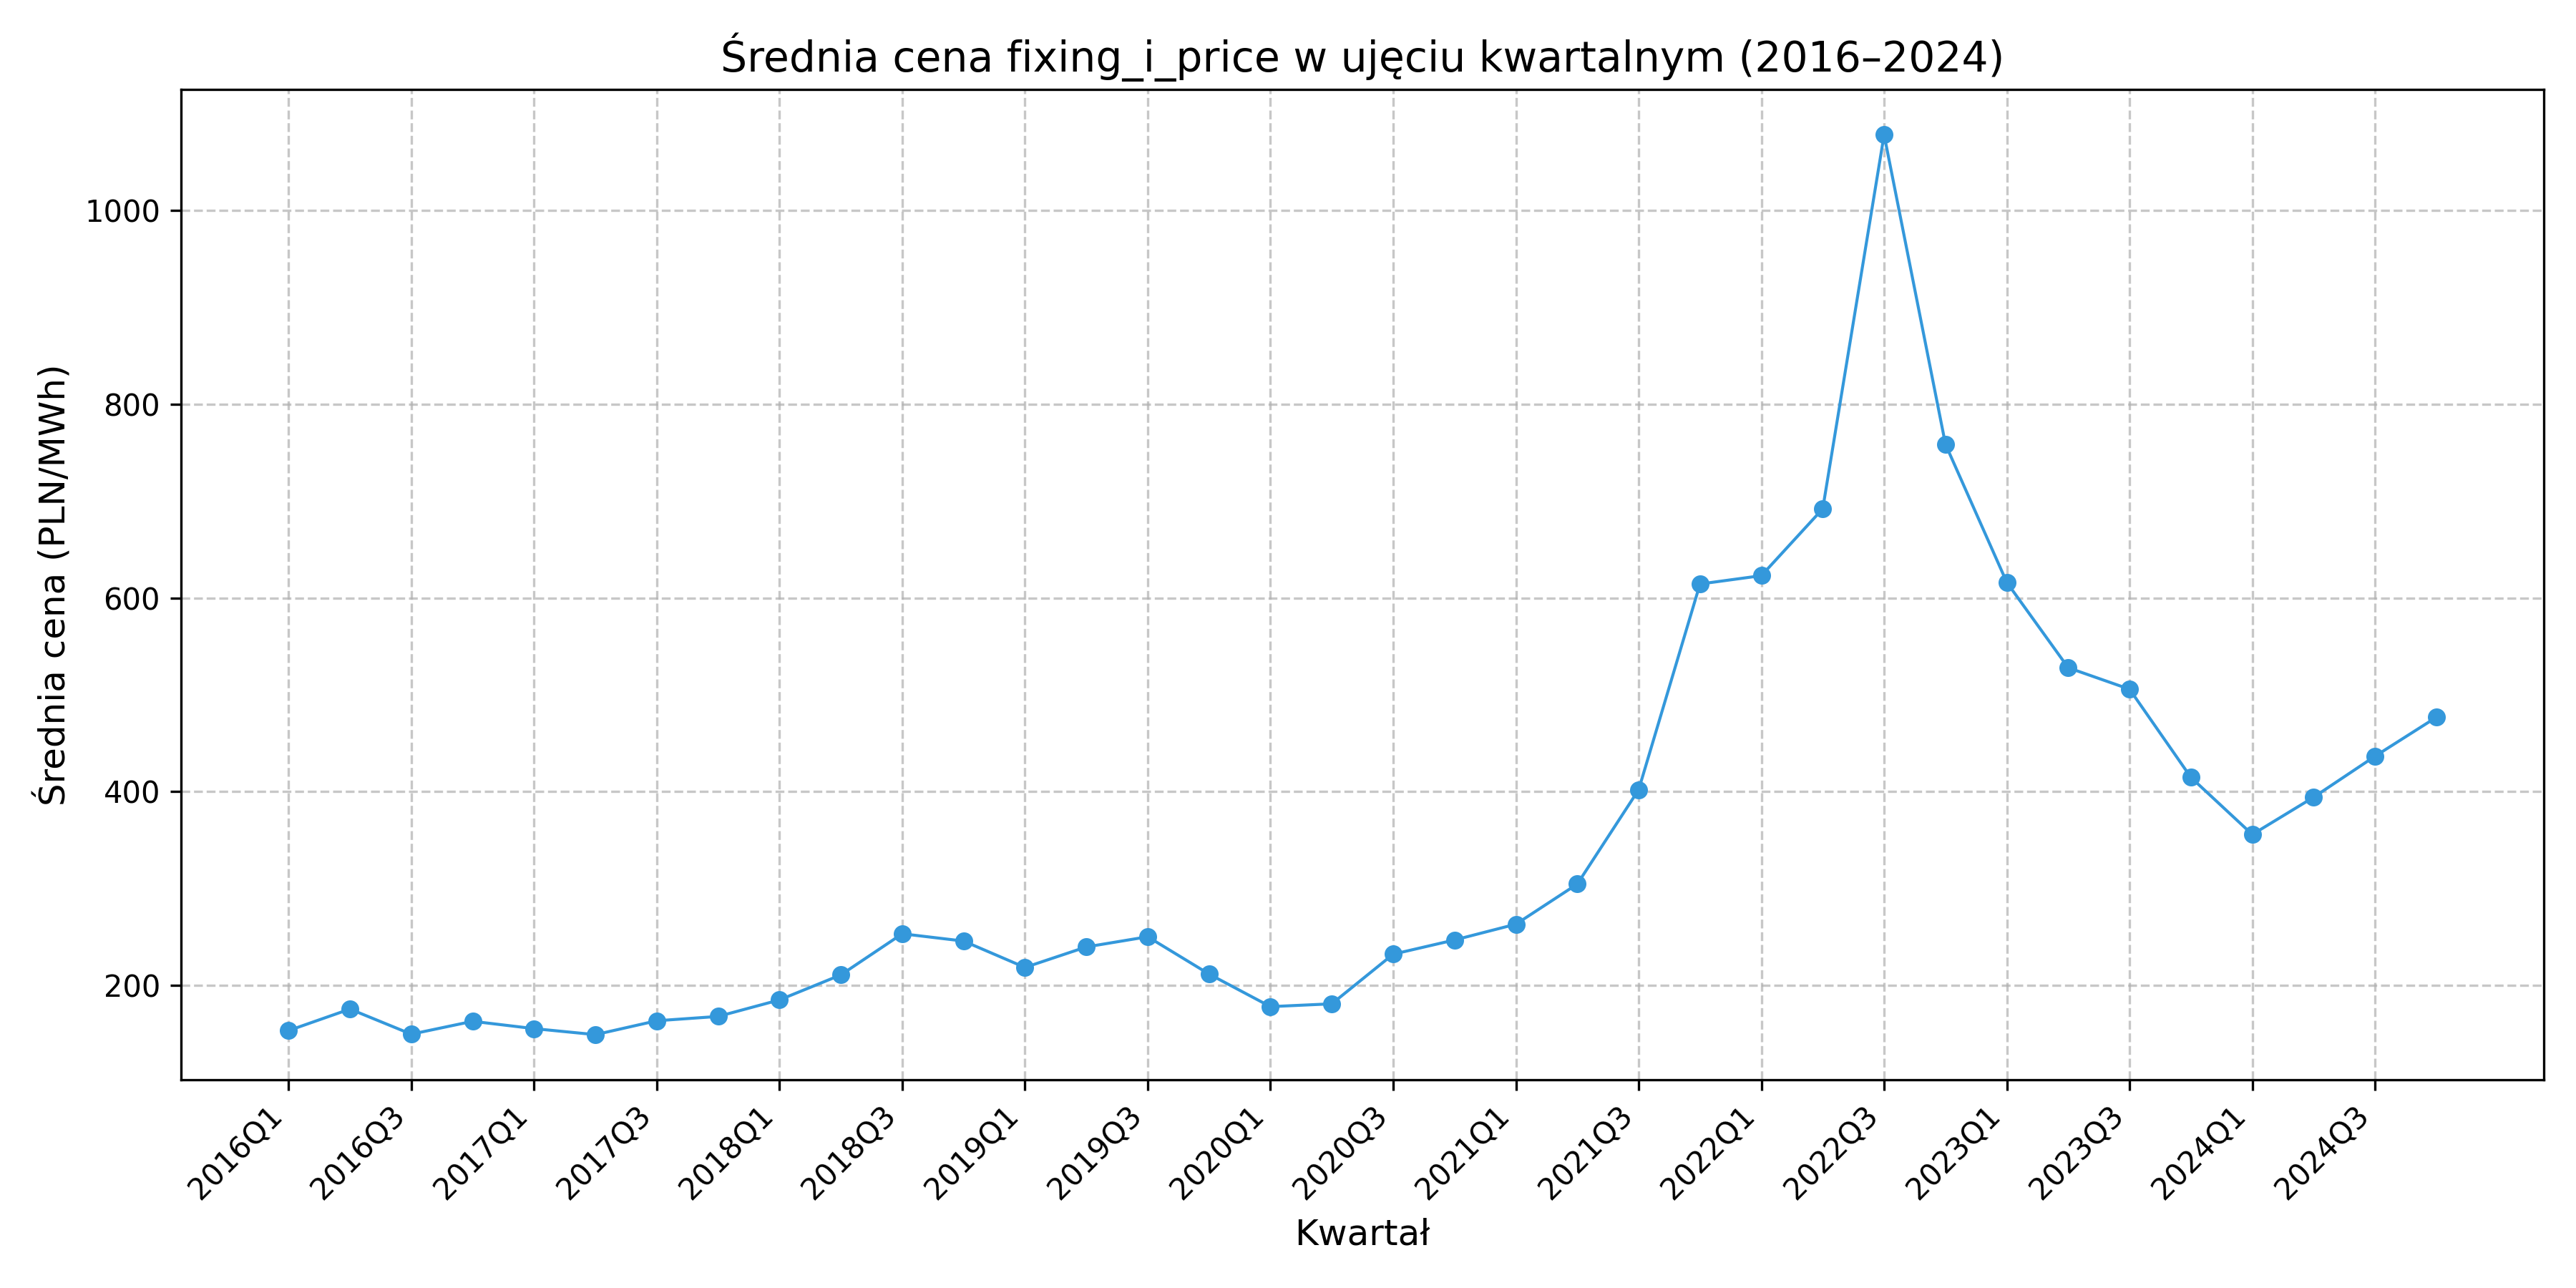
\includegraphics[width=\textwidth]{../plots/quarterly_fixing_i_price.png}
    \caption{Zmienność cen energii elektrycznej na RDN w latach 2016–2024}
    \label{fig:fixing-i-price-trend}
\end{figure}

Widać wyraźne różnice w poziomie cen w różnych okresach: od 2016 do Q4 roku 2020 ceny były stosunkowo stabilne, oscylując w przedziale 100–300 PLN/MWh. Sytuacja zmieniła się w 2020 roku, gdy zaczęły pojawiać się pierwsze skoki cenowe z powodu poważnych obostrzeń z powodu pandemii, a w 2022 roku, w wyniku kryzysu energetycznego wywołanego wojną na Ukrainie i ograniczeniami w dostawach paliw kopalnych, ceny osiągnęły rekordowe poziomy. Pierwszy okres zostanie określony jako okres stabilności cenowej, a drugi jako okres skoków cenowych. Te dwa okresy pokazują, jak niekorzystne sytuacje gospodarcze mogą wpływać na dynamikę cen energii, co ma istotne implikacje dla modelowania i prognozowania.

\begin{figure}
    \centering
    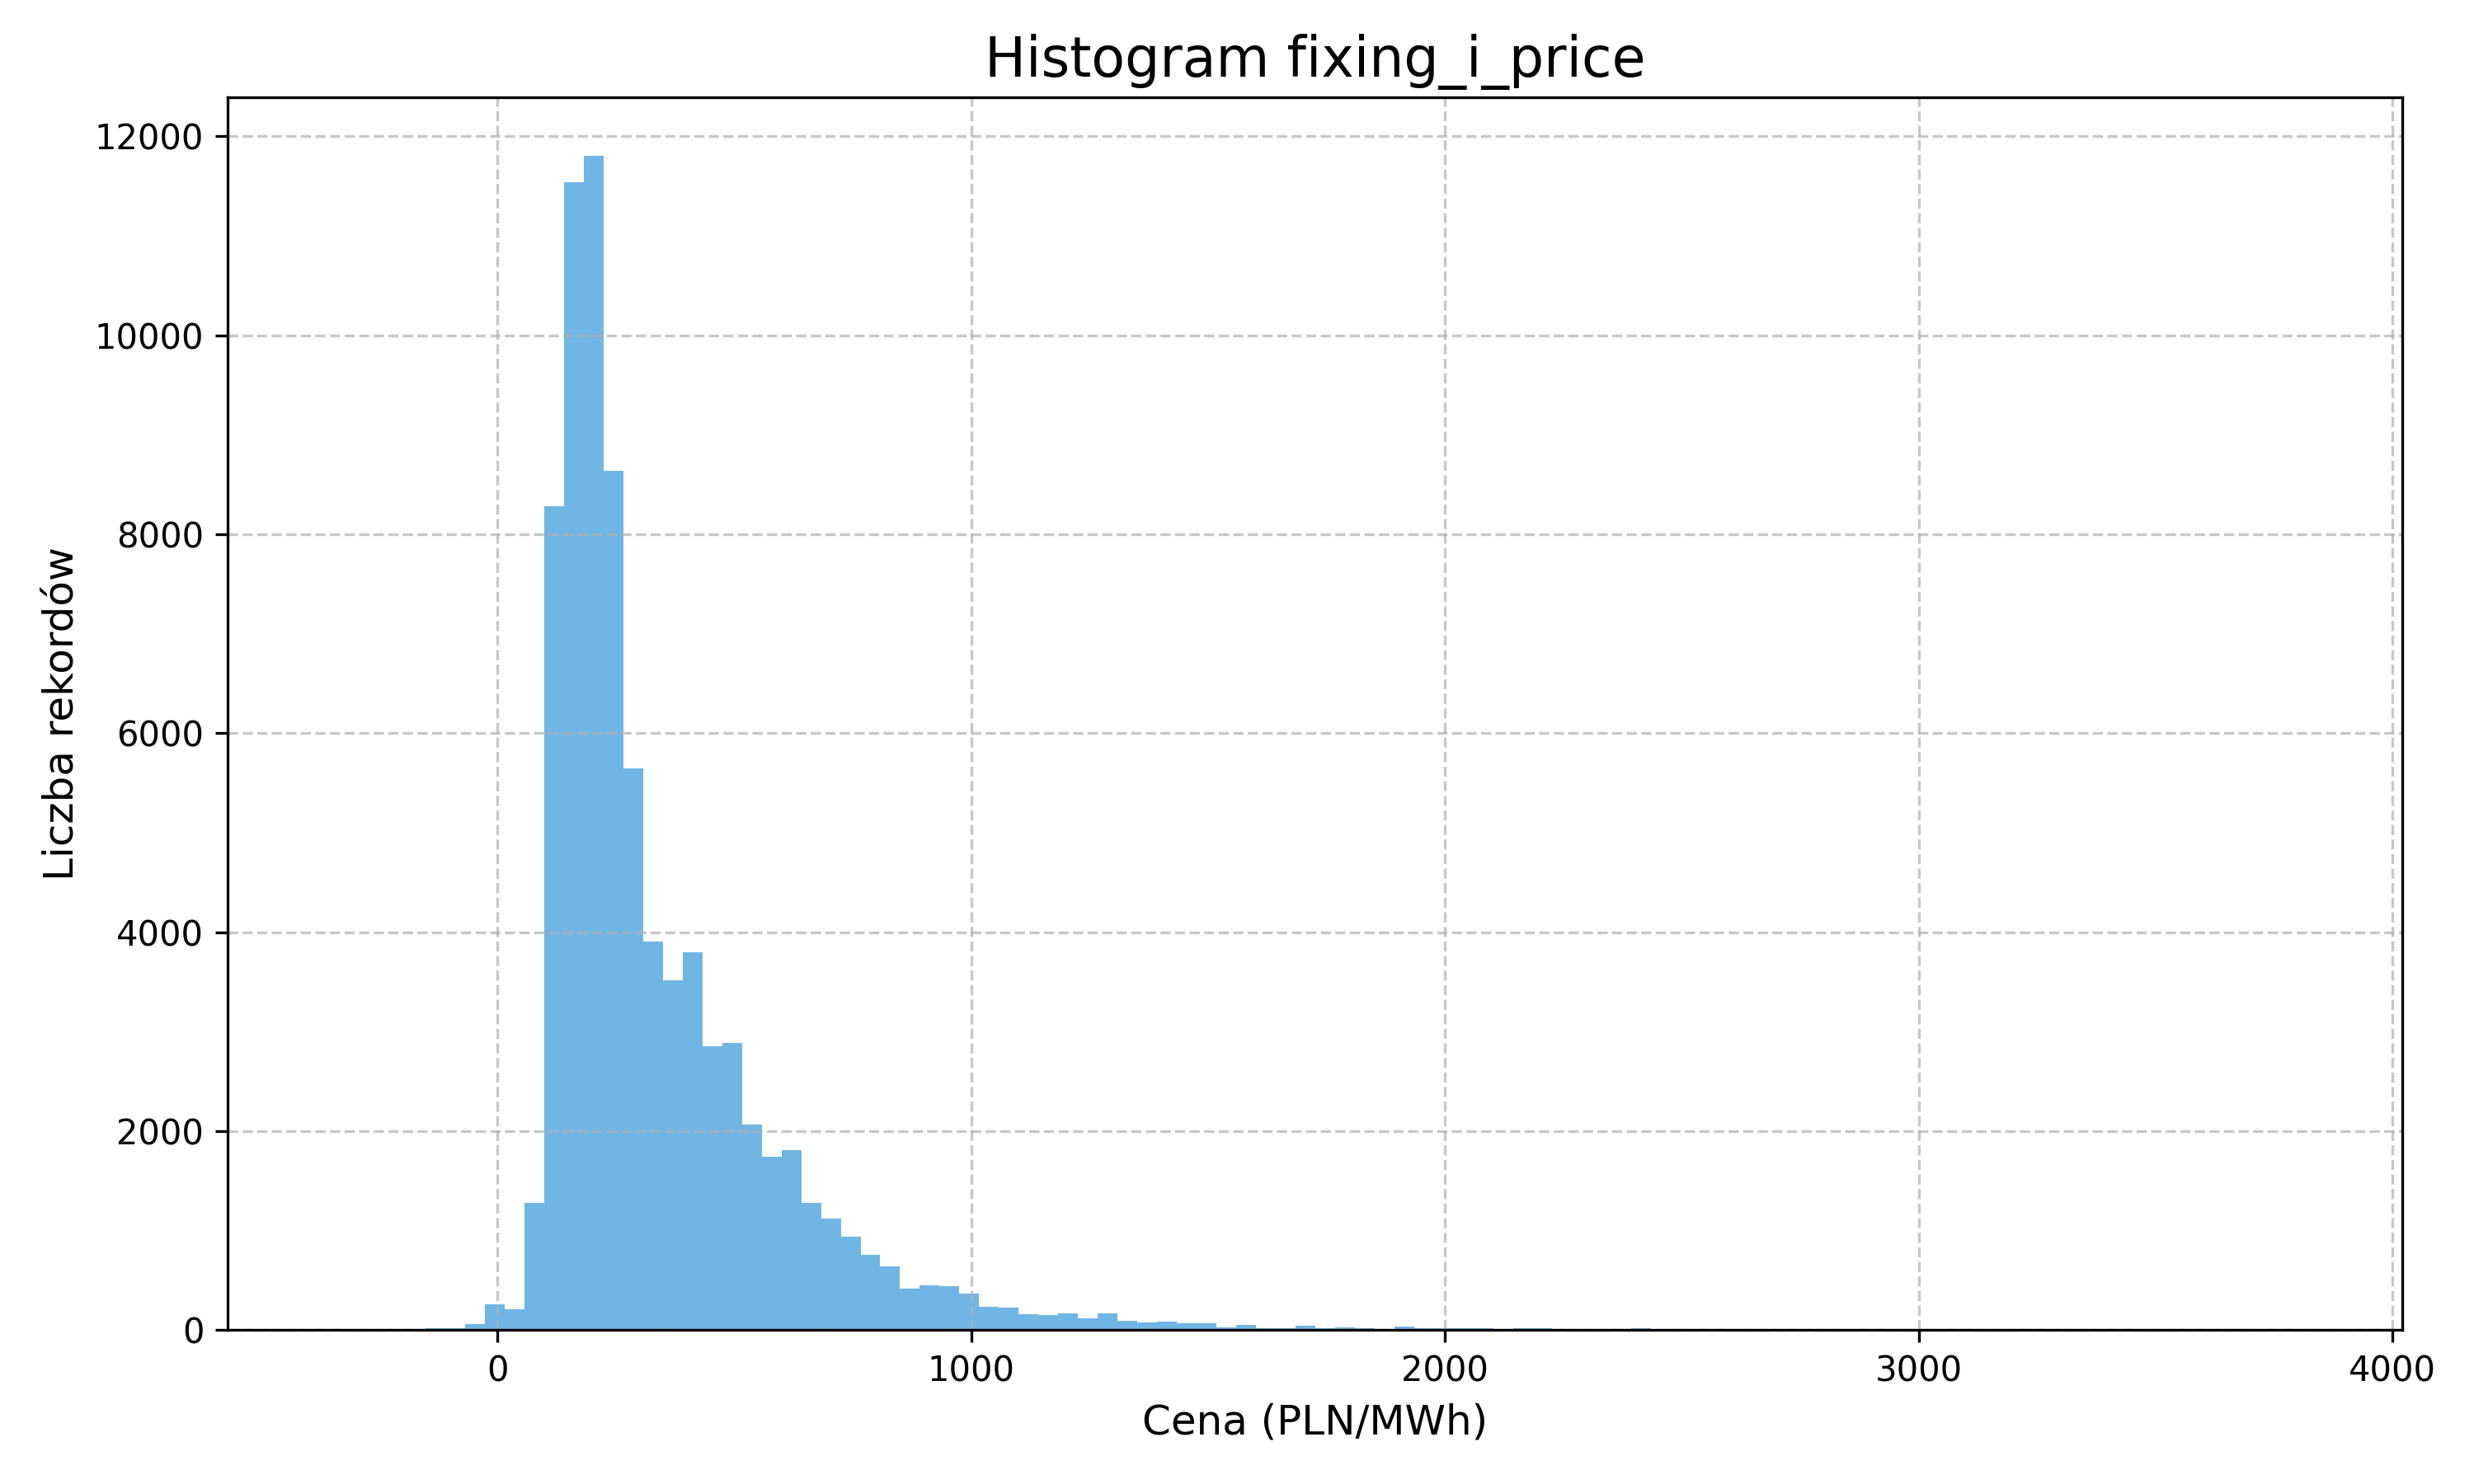
\includegraphics[width=\textwidth]{../plots/fixing_i_price_histogram.png}
    \caption{Histogram rozkładu zmiennej fixing\_i\_price}
    \label{fig:fixing-i-price-histogram}
\end{figure}

Rysunek \ref{fig:fixing-i-price-histogram} przedstawia histogram rozkładu zmiennej \texttt{fixing\_i\_price}. Rozkład jest wyraźnie asymetryczny, z długim prawym ogonem, co odzwierciedla występowanie skoków cenowych, takich jak te w 2022 roku. Ujemne ceny, choć rzadkie (ok. 0,4\% rekordów), są widoczne w lewej części histogramu, co potwierdza specyficzne cechy danych i potrzebę stosowania odpowiednich metod modelowania.

\section{Zbiór zmiennych niezależnych}
Dobór zmiennych niezależnych jest bardzo ważny dla osiągnięcia dobrych wyników badania. W niniejszej pracy wykorzystano różnorodne zmienne niezależne, które można podzielić na kilka kategorii. Obejmują one dane pogodowe, zapotrzebowanie, straty sieciowe, bilanse wymiany transgranicznej, dane o produkcji energii przez poszczególne typy generatorów, ceny paliw kopalnych, emisji CO$_2$ i inne. Wybór tych zmiennych oparty jest na ich potencjalnym wpływie na ceny energii elektrycznej. Poniżej przedstawiono szczegółowy opis każdej z kategorii zmiennych niezależnych, które zostały uwzględnione w analizie.

\subsection{Dane pogodowe}
Pierwotnie zbiór danych miał być zestawiony z danych dostępnych za pomocą oficjalnej strony Instytutu Meteorologii i Gospodarki Wodnej, natomiat dane historyczne z lat 2016-2024 mają ograniczoną rozdzielczość. Zbierane są przez wiele stacji meteorologicznych, które są rozproszone po całym kraju, ale tylko w godzinach 6:00, 12:00 oraz 18:00. Aproksymować dane pogodowe w godzinach nocnych jest zadaniem nie do wykonania, szczególnie w przypadku sezonów zimowych, gdzie temperatura w nocy może drastycznie spadać w ciągu godziny. Z tego powodu jako źródło danych pogodowych wykorzystano stronę open-meteo.com \cite{METEO}. Jest to strona, która zbiera dane z różnych stacji meteorologicznych i udostępnia je w formie API. Dzięki temu można pobrać dane pogodowe dla dowolnego okresu czasu i lokalizacji.

Dane pogodowe zostały pobrane dla czterech lokalizacji w Polsce: Warszawy (WAW), Koszalina (KSZ), Krakowa (KRK) i Babimost (BAB), a następnie dopasowane do godzinowego formatu danych RDN, co pozwoliło na ich integrację z pozostałymi zmiennymi. Wybór miast został podyktowany ich zróżnicowaniem geograficznym i klimatycznym, co pozwala uwzględnić regionalne różnice w warunkach pogodowych wpływających na produkcję i zapotrzebowanie na energię. Warszawa, jako stolica i największe miasto Polski, reprezentuje centralny region kraju o wysokim zapotrzebowaniu na energię, szczególnie w okresach zimowych i letnich. Koszalin, położony na Pomorzu, jest kluczowy ze względu na bliskość farm wiatrowych na Morzu Bałtyckim, co czyni go istotnym punktem dla analizy produkcji energii wiatrowej. Kraków, znajdujący się w południowej Polsce, charakteryzuje się większym udziałem energii słonecznej w miksie energetycznym, a także wysokim zapotrzebowaniem na energię w sezonie grzewczym z powodu zanieczyszczenia powietrza i częstego stosowania ogrzewania elektrycznego. Babimost, zlokalizowany w zachodniej Polsce, jest istotny ze względu na swoje położenie w pobliżu granicy z Niemcami.

Parametry pogodowe zostały wybrane z uwzględnieniem ich bezpośredniego wpływu na rynek energii. Temperatura jest kluczowym czynnikiem, ponieważ wpływa na zapotrzebowanie na energię – niskie temperatury zwiększają zużycie energii na ogrzewanie, natomiast wysokie temperatury latem podnoszą zapotrzebowanie na klimatyzację. Prędkość wiatru mierzona na wysokości 100 metrów nad powierzchnią ziemi została wybrana, ponieważ jest to przeciętna wysokość dla turbin wiatrowych w Polsce, co pozwala dokładniej oszacować potencjalną produkcję energii z farm wiatrowych. Promieniowanie słoneczne jest istotne dla produkcji energii z paneli fotowoltaicznych. Zachmurzenie zostało uwzględnione, ponieważ wysoki poziom zachmurzenia zmniejsza efektywność paneli słonecznych, co może zwiększać ceny energii poprzez ograniczenie podaży z OZE. Wybór tych parametrów pozwala na kompleksową analizę wpływu pogody na ceny energii na RDN.

Poniżej przedstawię wykresy dla każdego z parametrów pogodowych, które zostały uwzględnione w analizie. Wykresy przedstawiają zmienność danych pogodowych w czasie. Zachmurzenie jest wyrażone w oktantach (0-8), gdzie 0 oznacza brak zachmurzenia, a 8 oznacza całkowite zachmurzenie.

\begin{figure}[H]
    \centering
    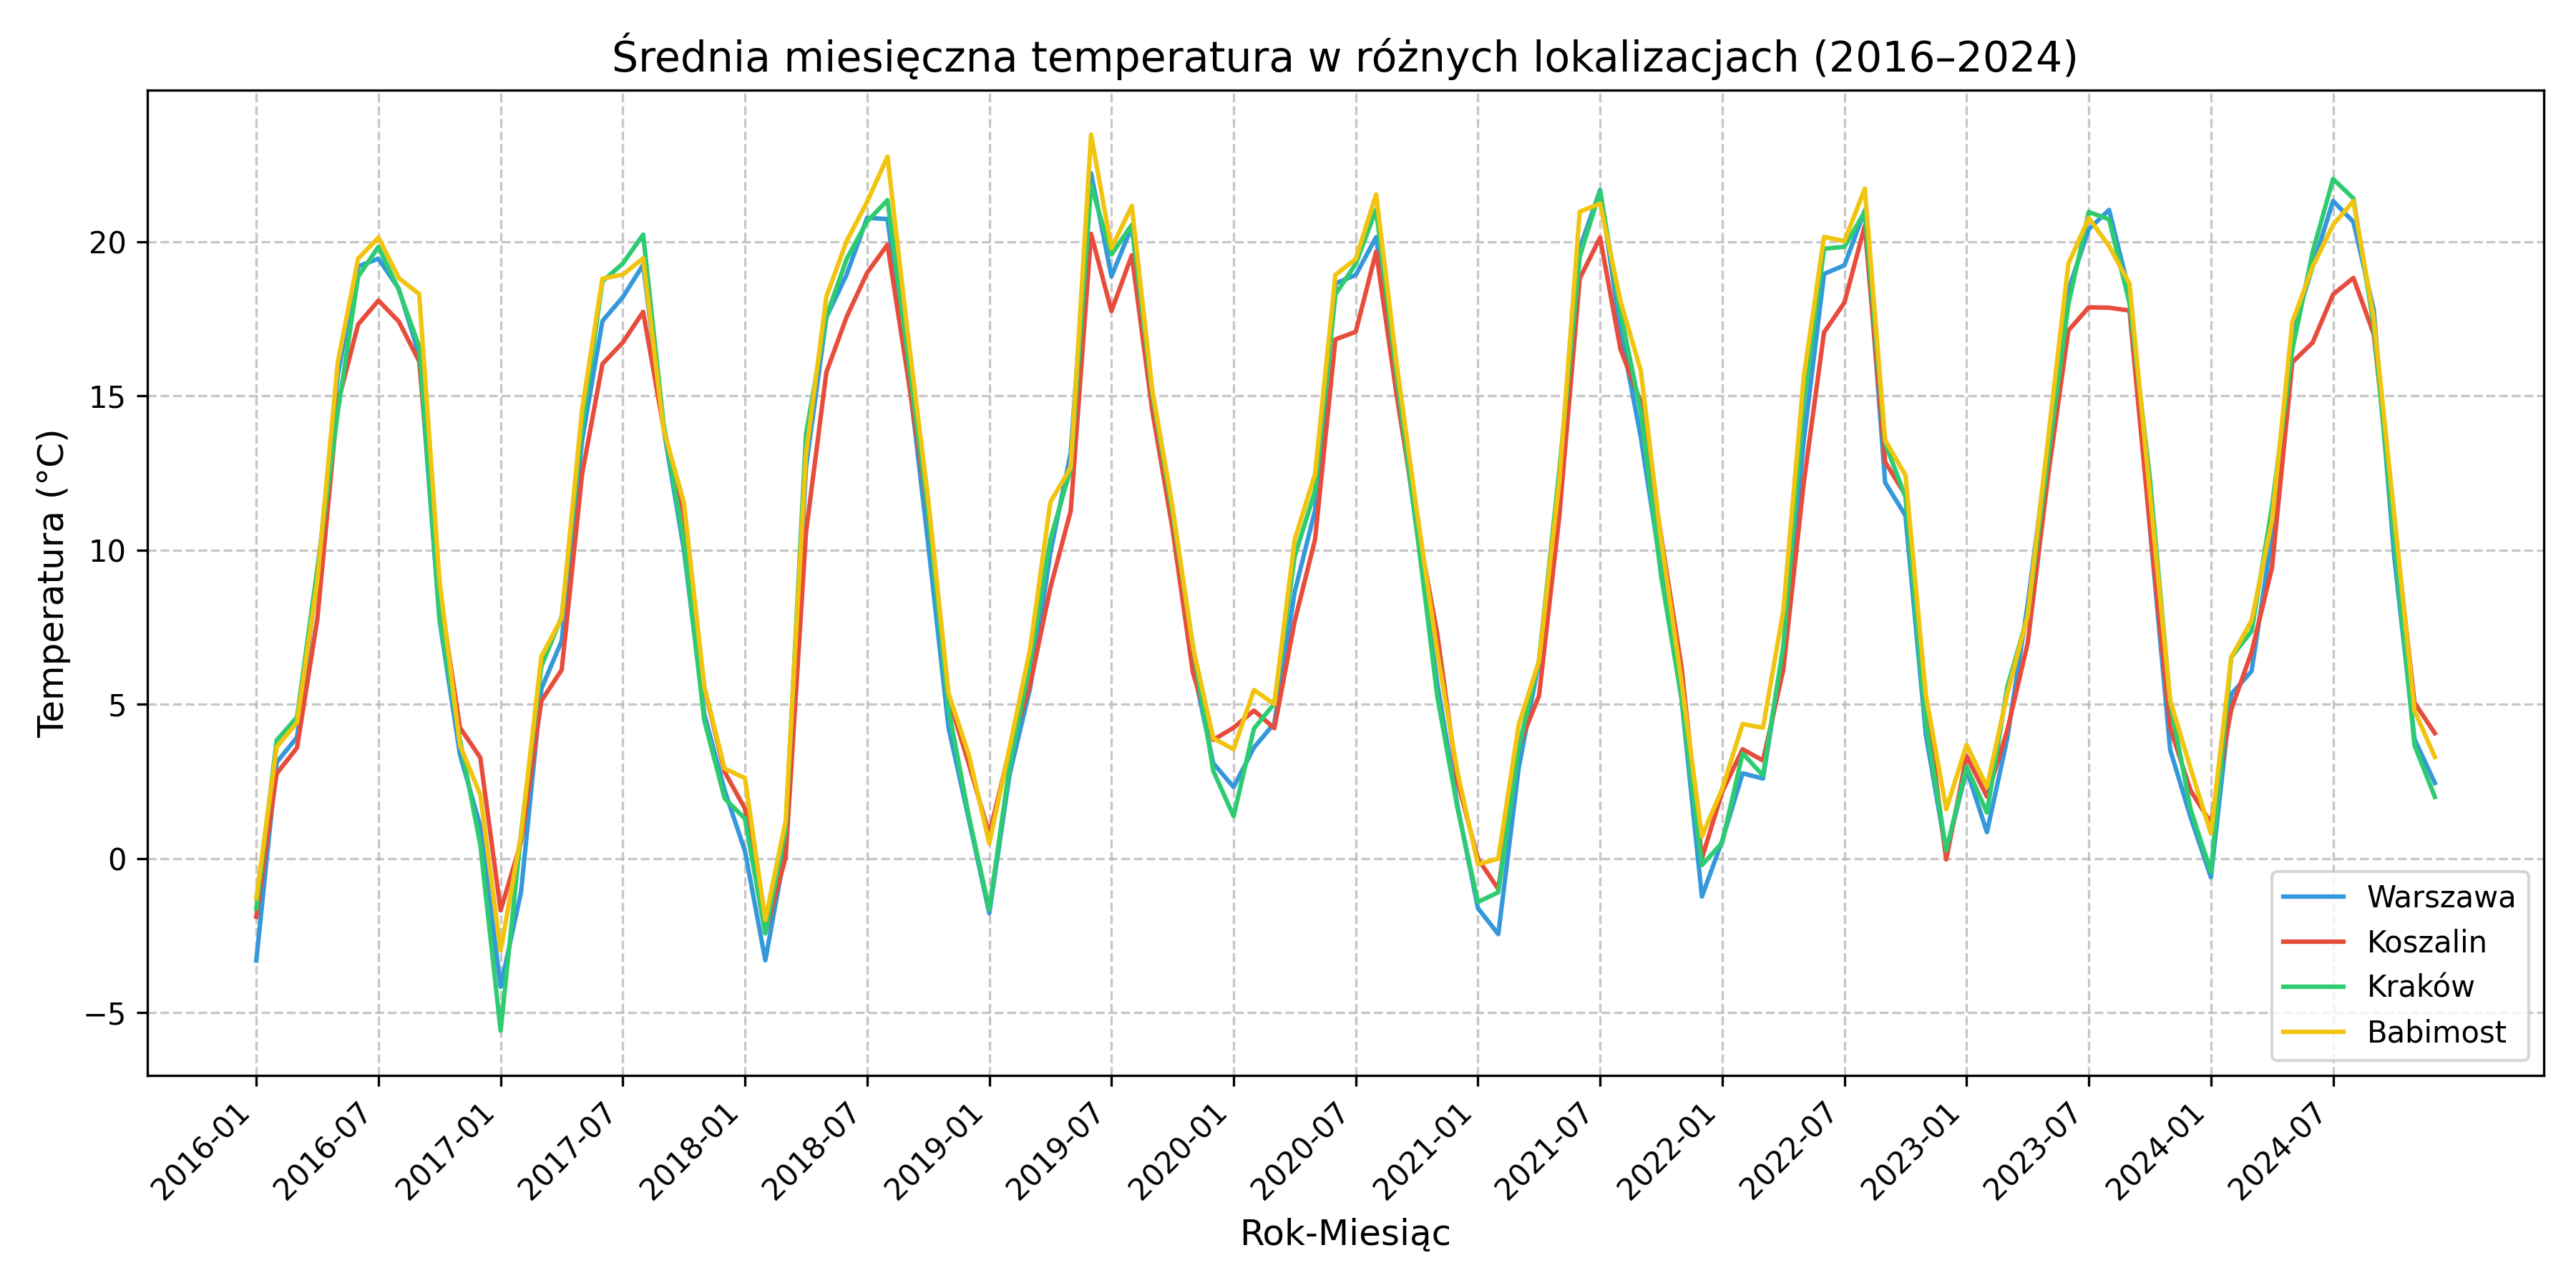
\includegraphics[width=\textwidth]{../plots/weather/temp_time_series_full.png}
    \caption{Zmienność temperatury w czasie (2016–2024)}
    \label{fig:temp-time-series-full}
\end{figure}

\begin{figure}[H]
    \centering
    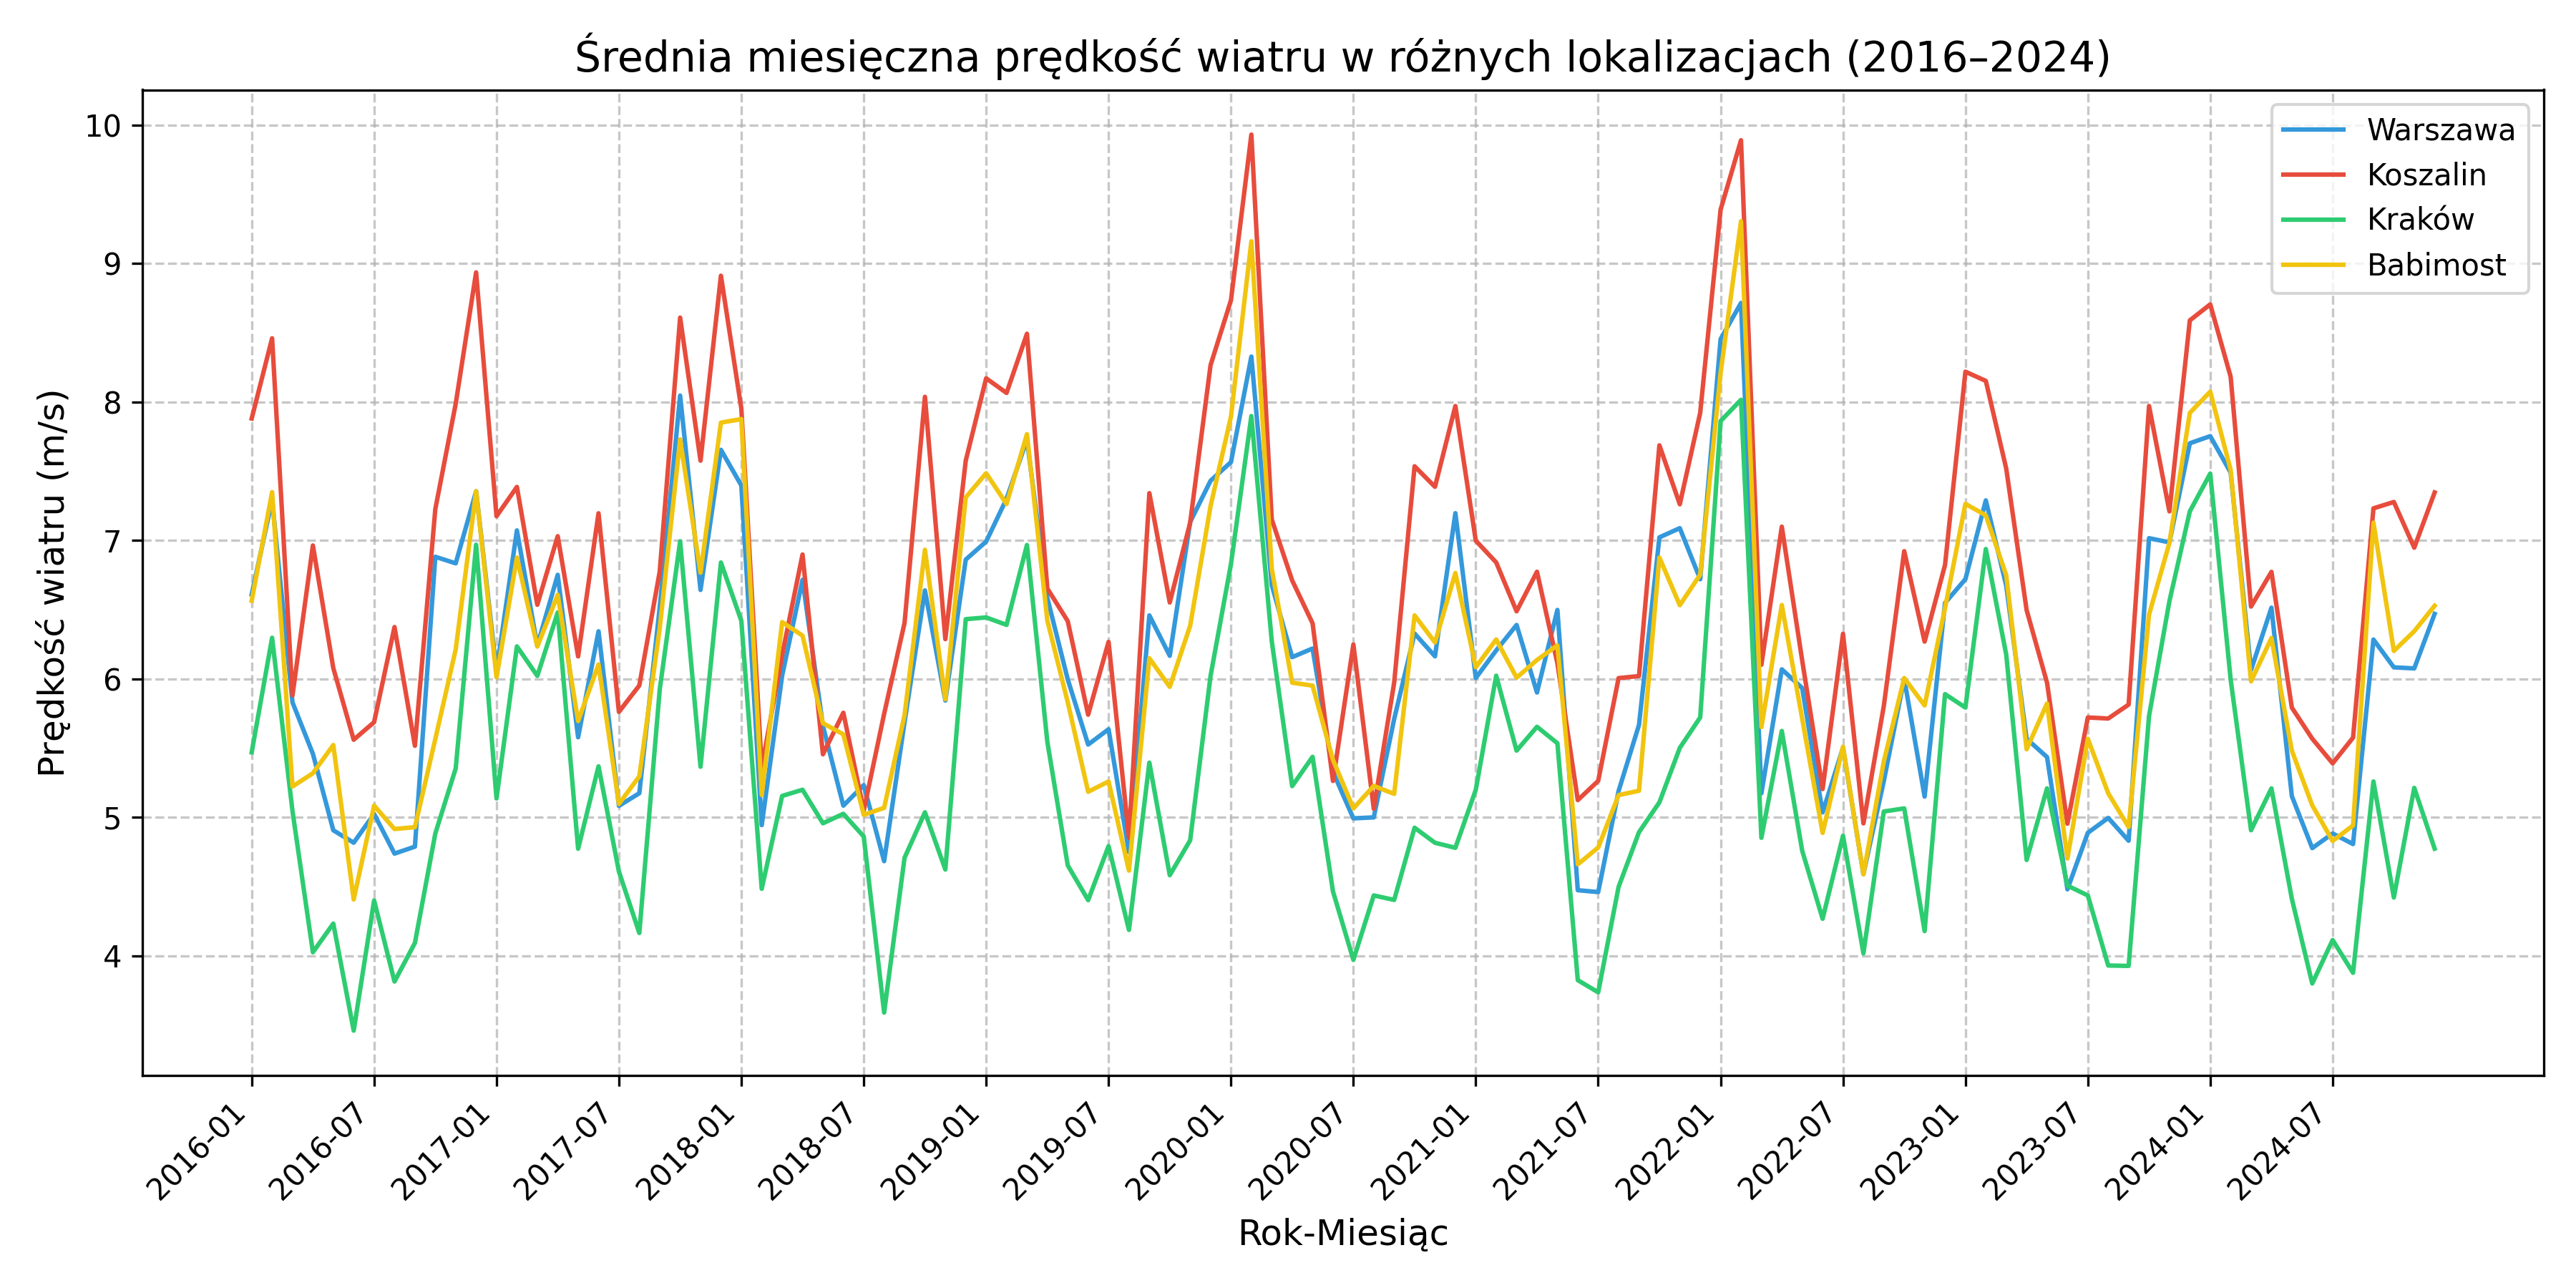
\includegraphics[width=\textwidth]{../plots/weather/wind_speed_time_series_full.png}
    \caption{Zmienność prędkości wiatru w czasie (2016–2024)}
    \label{fig:wind-speed-time-series-full}
\end{figure}

\begin{figure}[H]
    \centering
    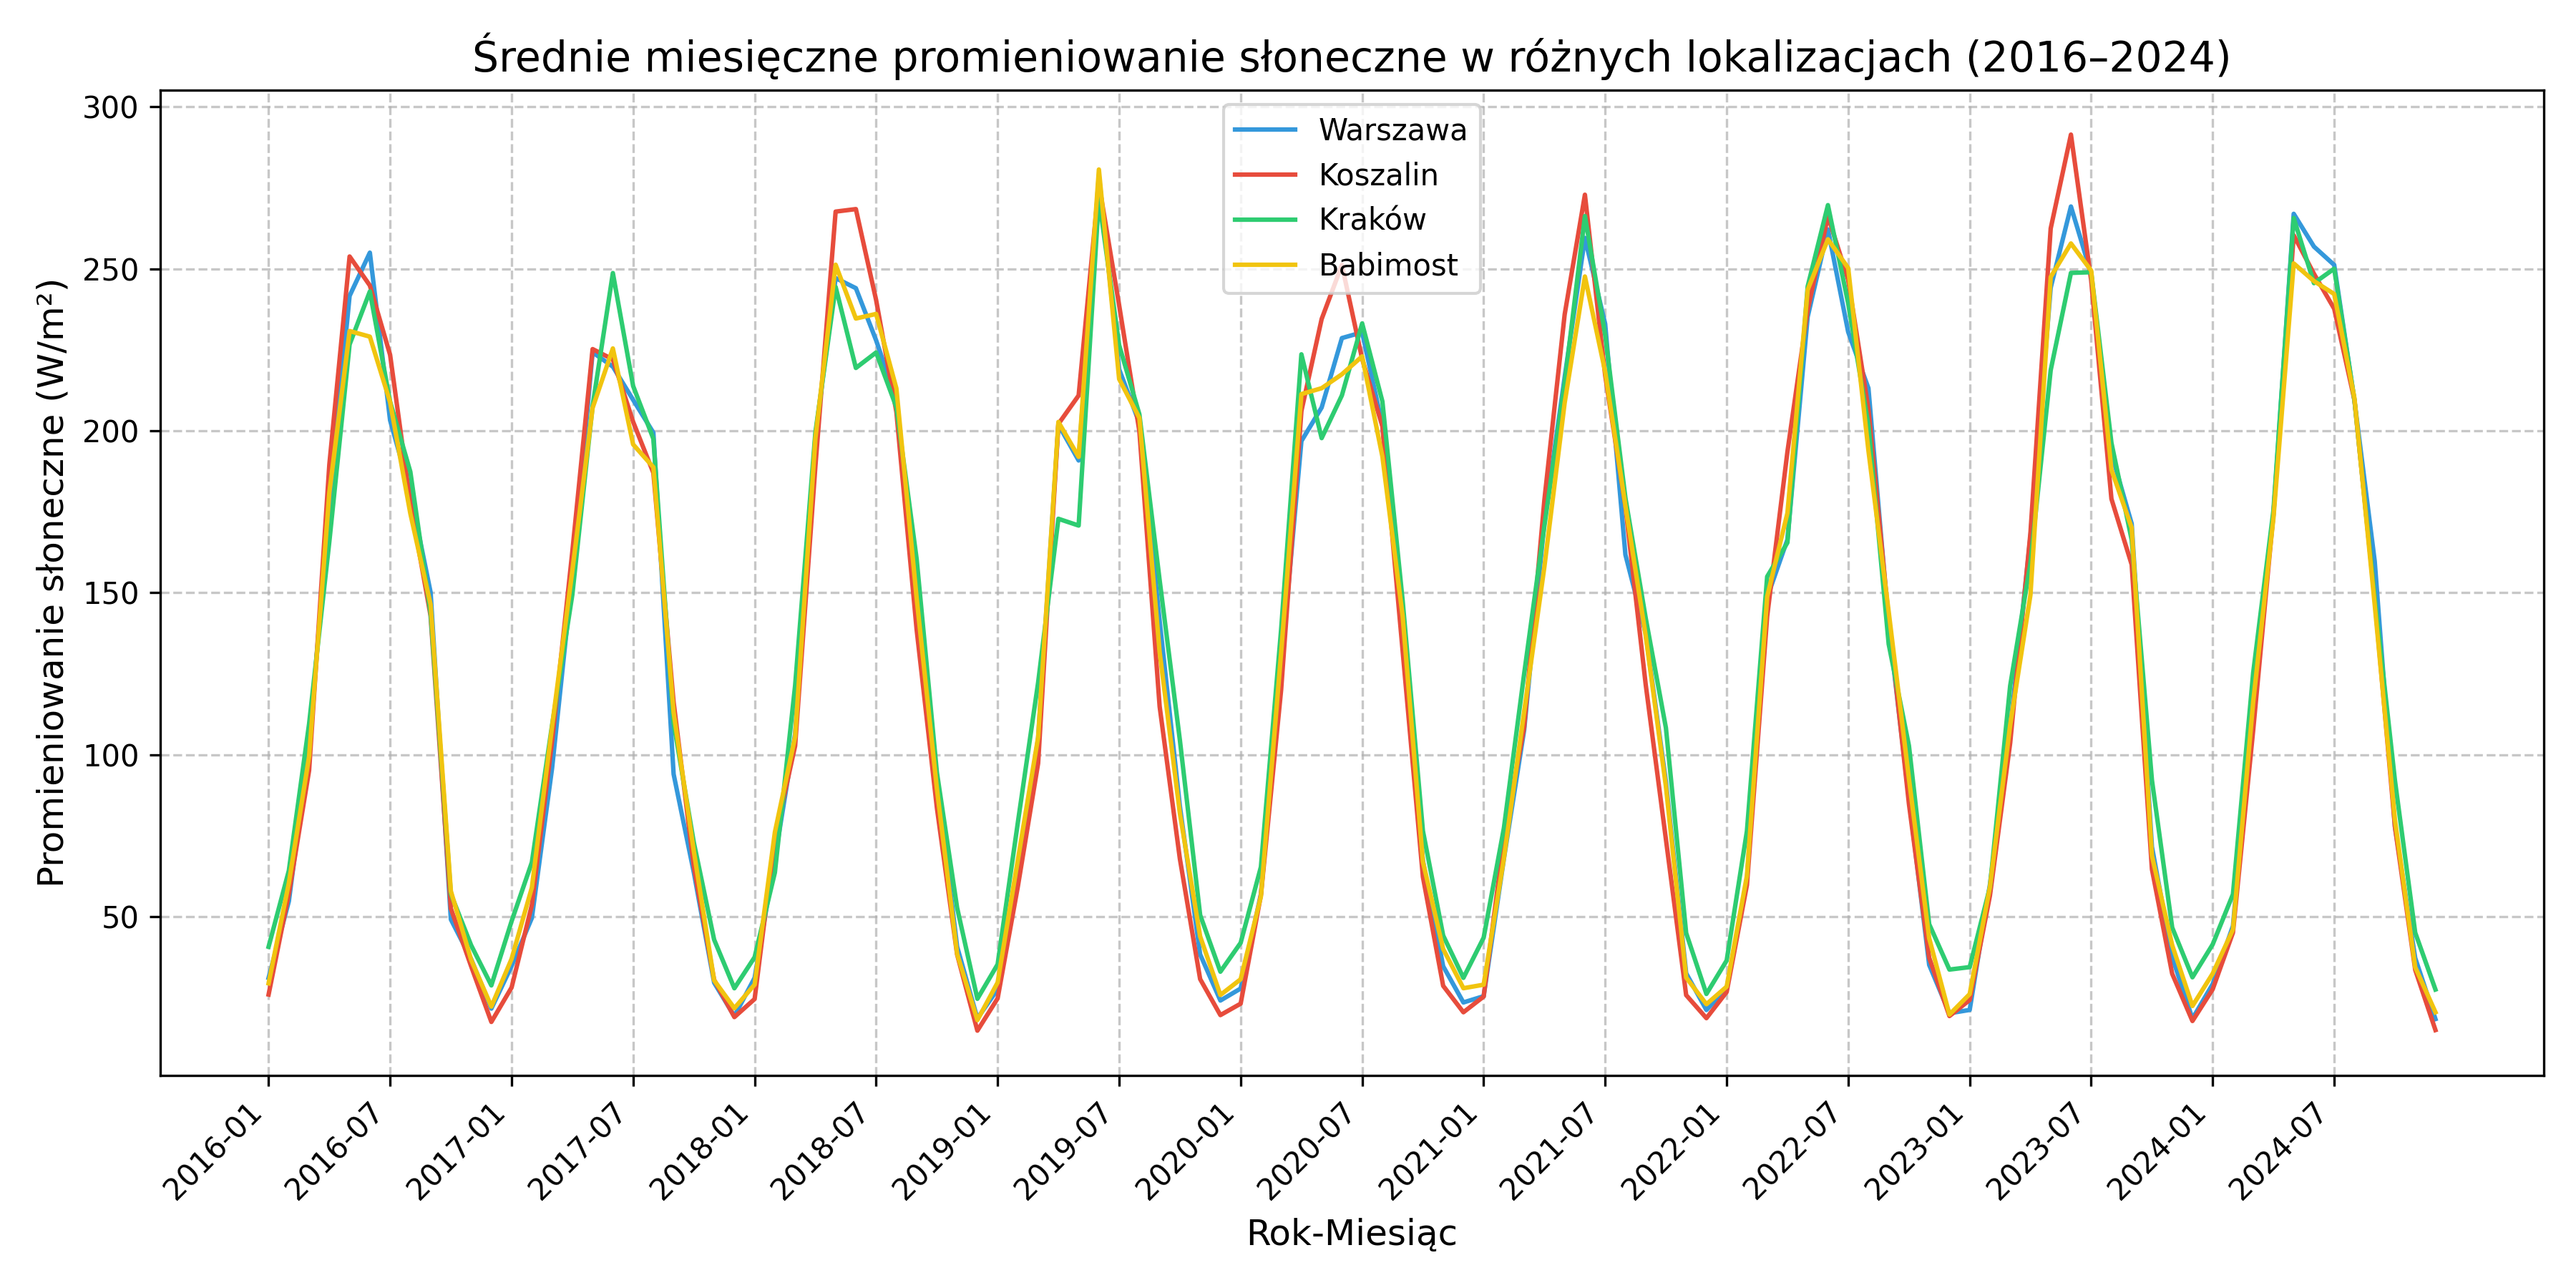
\includegraphics[width=\textwidth]{../plots/weather/solar_radiation_time_series_full.png}
    \caption{Zmienność promieniowania słonecznego w czasie (2016–2024)}
    \label{fig:solar-radiation-time-series-full}
\end{figure}

\begin{figure}[H]
    \centering
    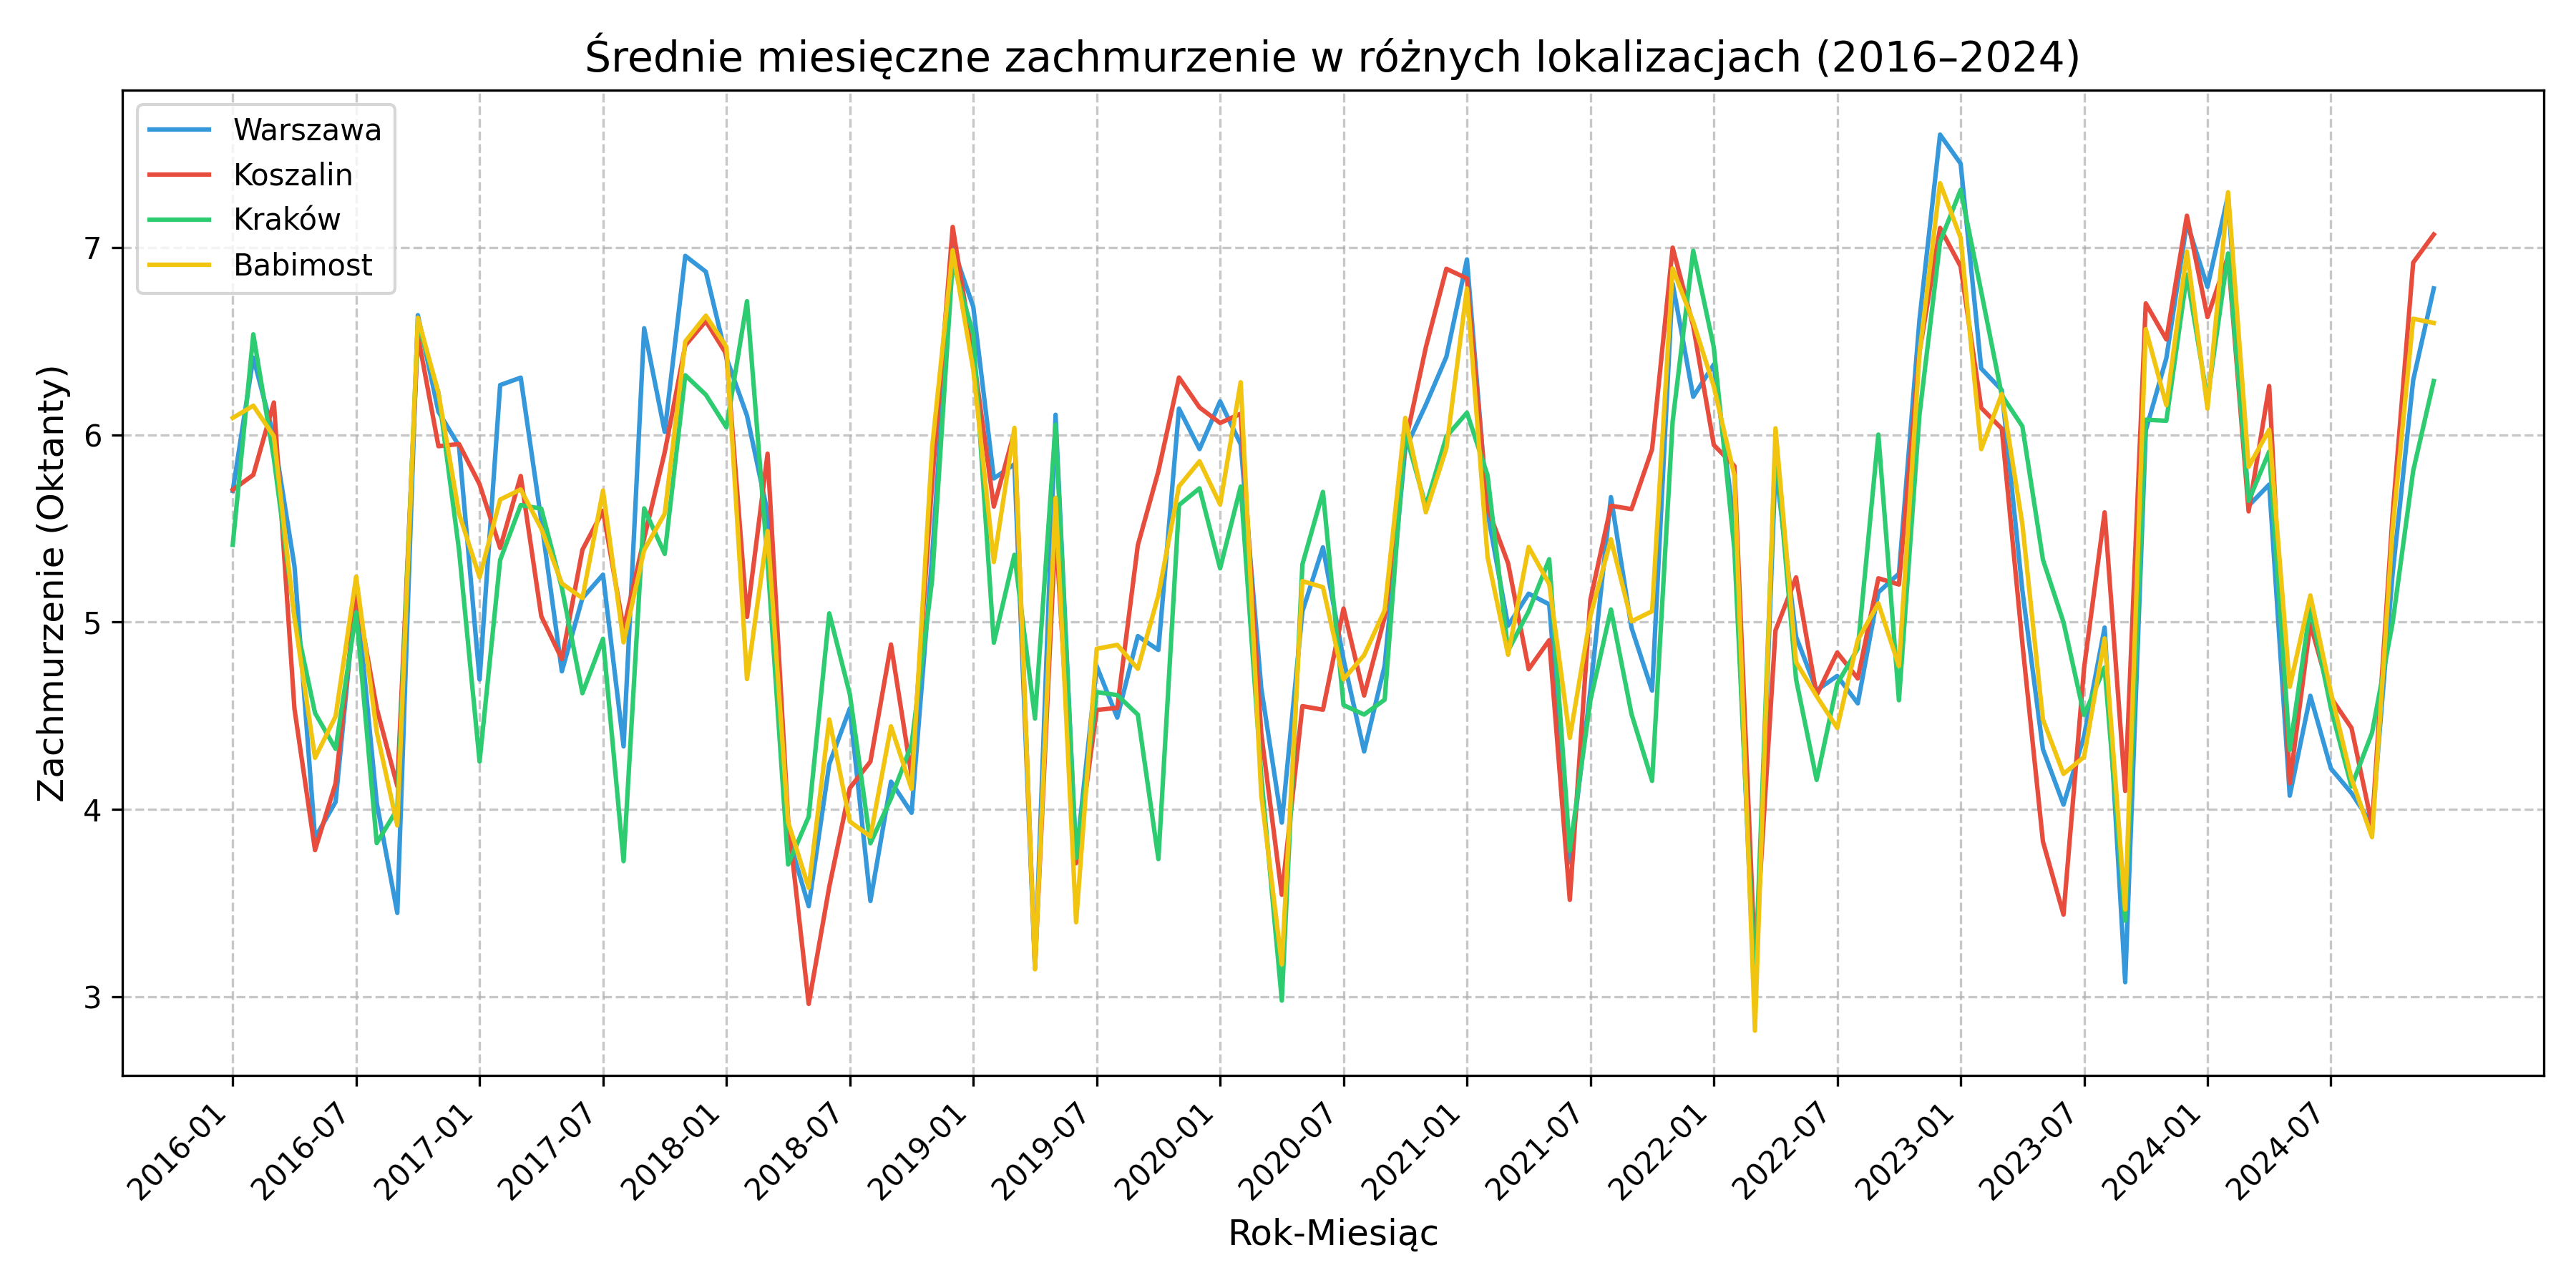
\includegraphics[width=\textwidth]{../plots/weather/cloud_cover_time_series_full.png}
    \caption{Zmienność zachmurzenia w czasie (2016–2024)}
    \label{fig:cloud-cover-time-series-full}
\end{figure}

Każdy z wykresów przedstawia zmienność danego parametru pogodowego w wybranych lokalizacjach w przeciągu okresu badawczego. Wyraźnie widać sezonowe wahania parametrów pogodowych, co jest typowe dla klimatu Polski. Temperatura i promieniowanie słoneczne mają wyraźnie większe wartości w sezonach letnich, prędkość wiatru w sezonach zimowych, a zachmurzenie ma bardziej zróżnicowany charakter.

Chciałbym również przybliżyć wykresy i potwierdzić efekt sezonowości na przykładzie 2022 roku. 

\begin{figure}[H]
    \centering
    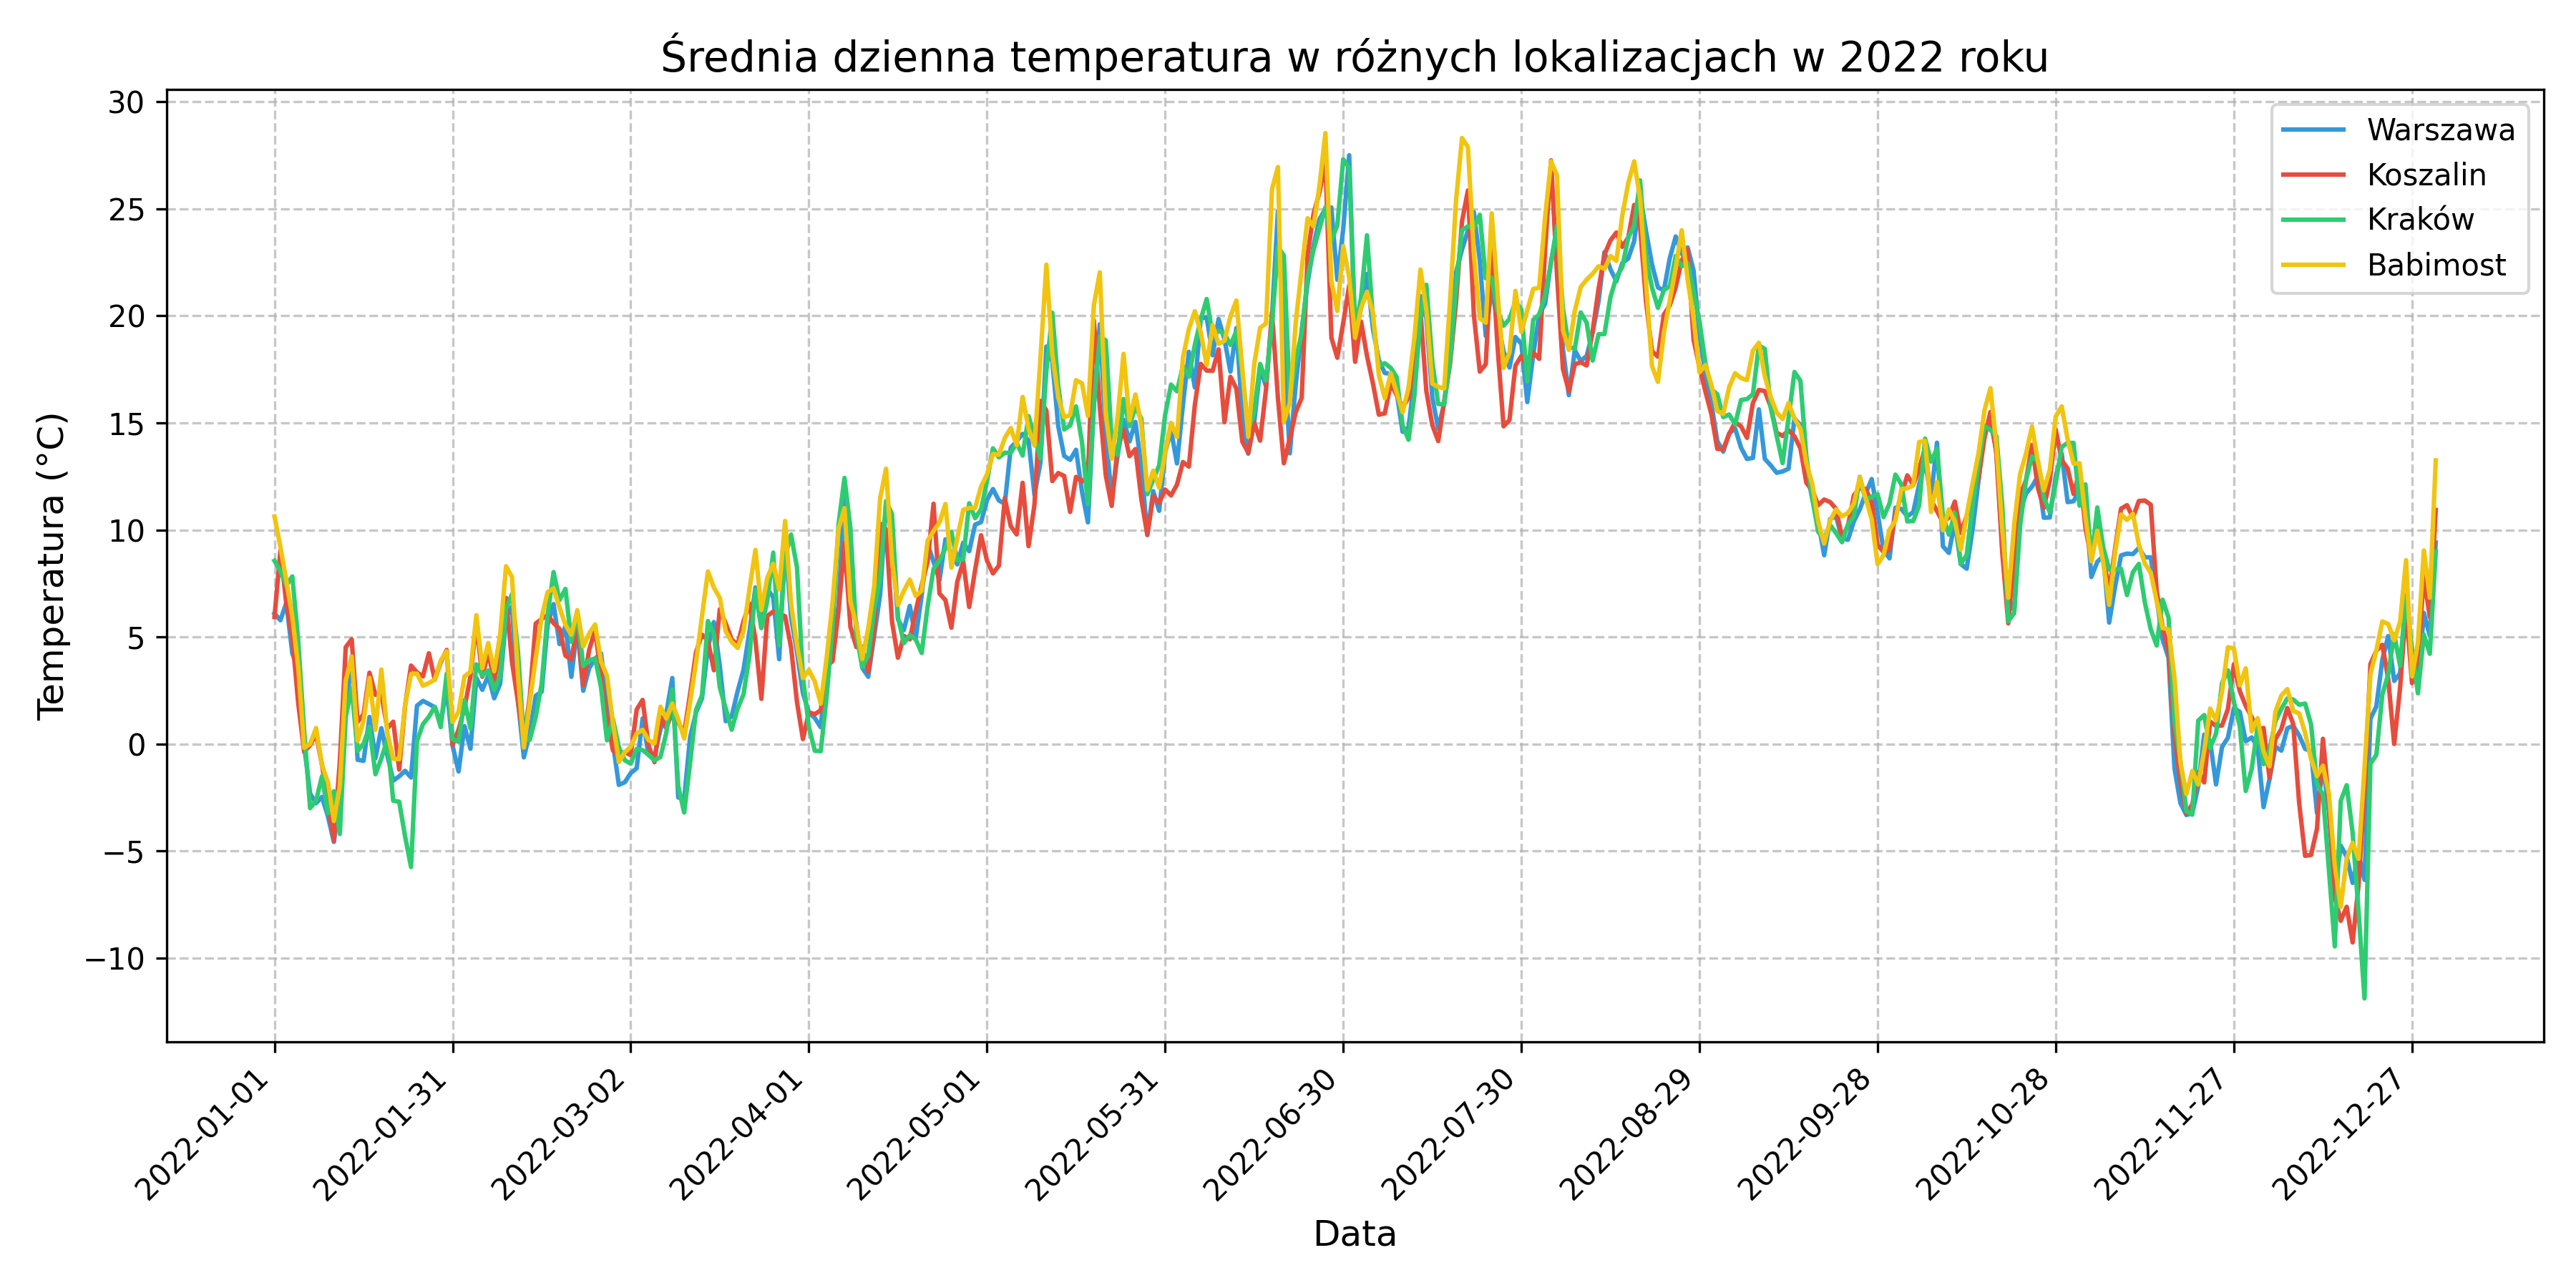
\includegraphics[width=\textwidth]{../plots/weather/temp_time_series_2022.png}
    \caption{Zmienność temperatury w czasie (2022)}
    \label{fig:temp-time-series-2022}
\end{figure}

\begin{figure}[H]
    \centering
    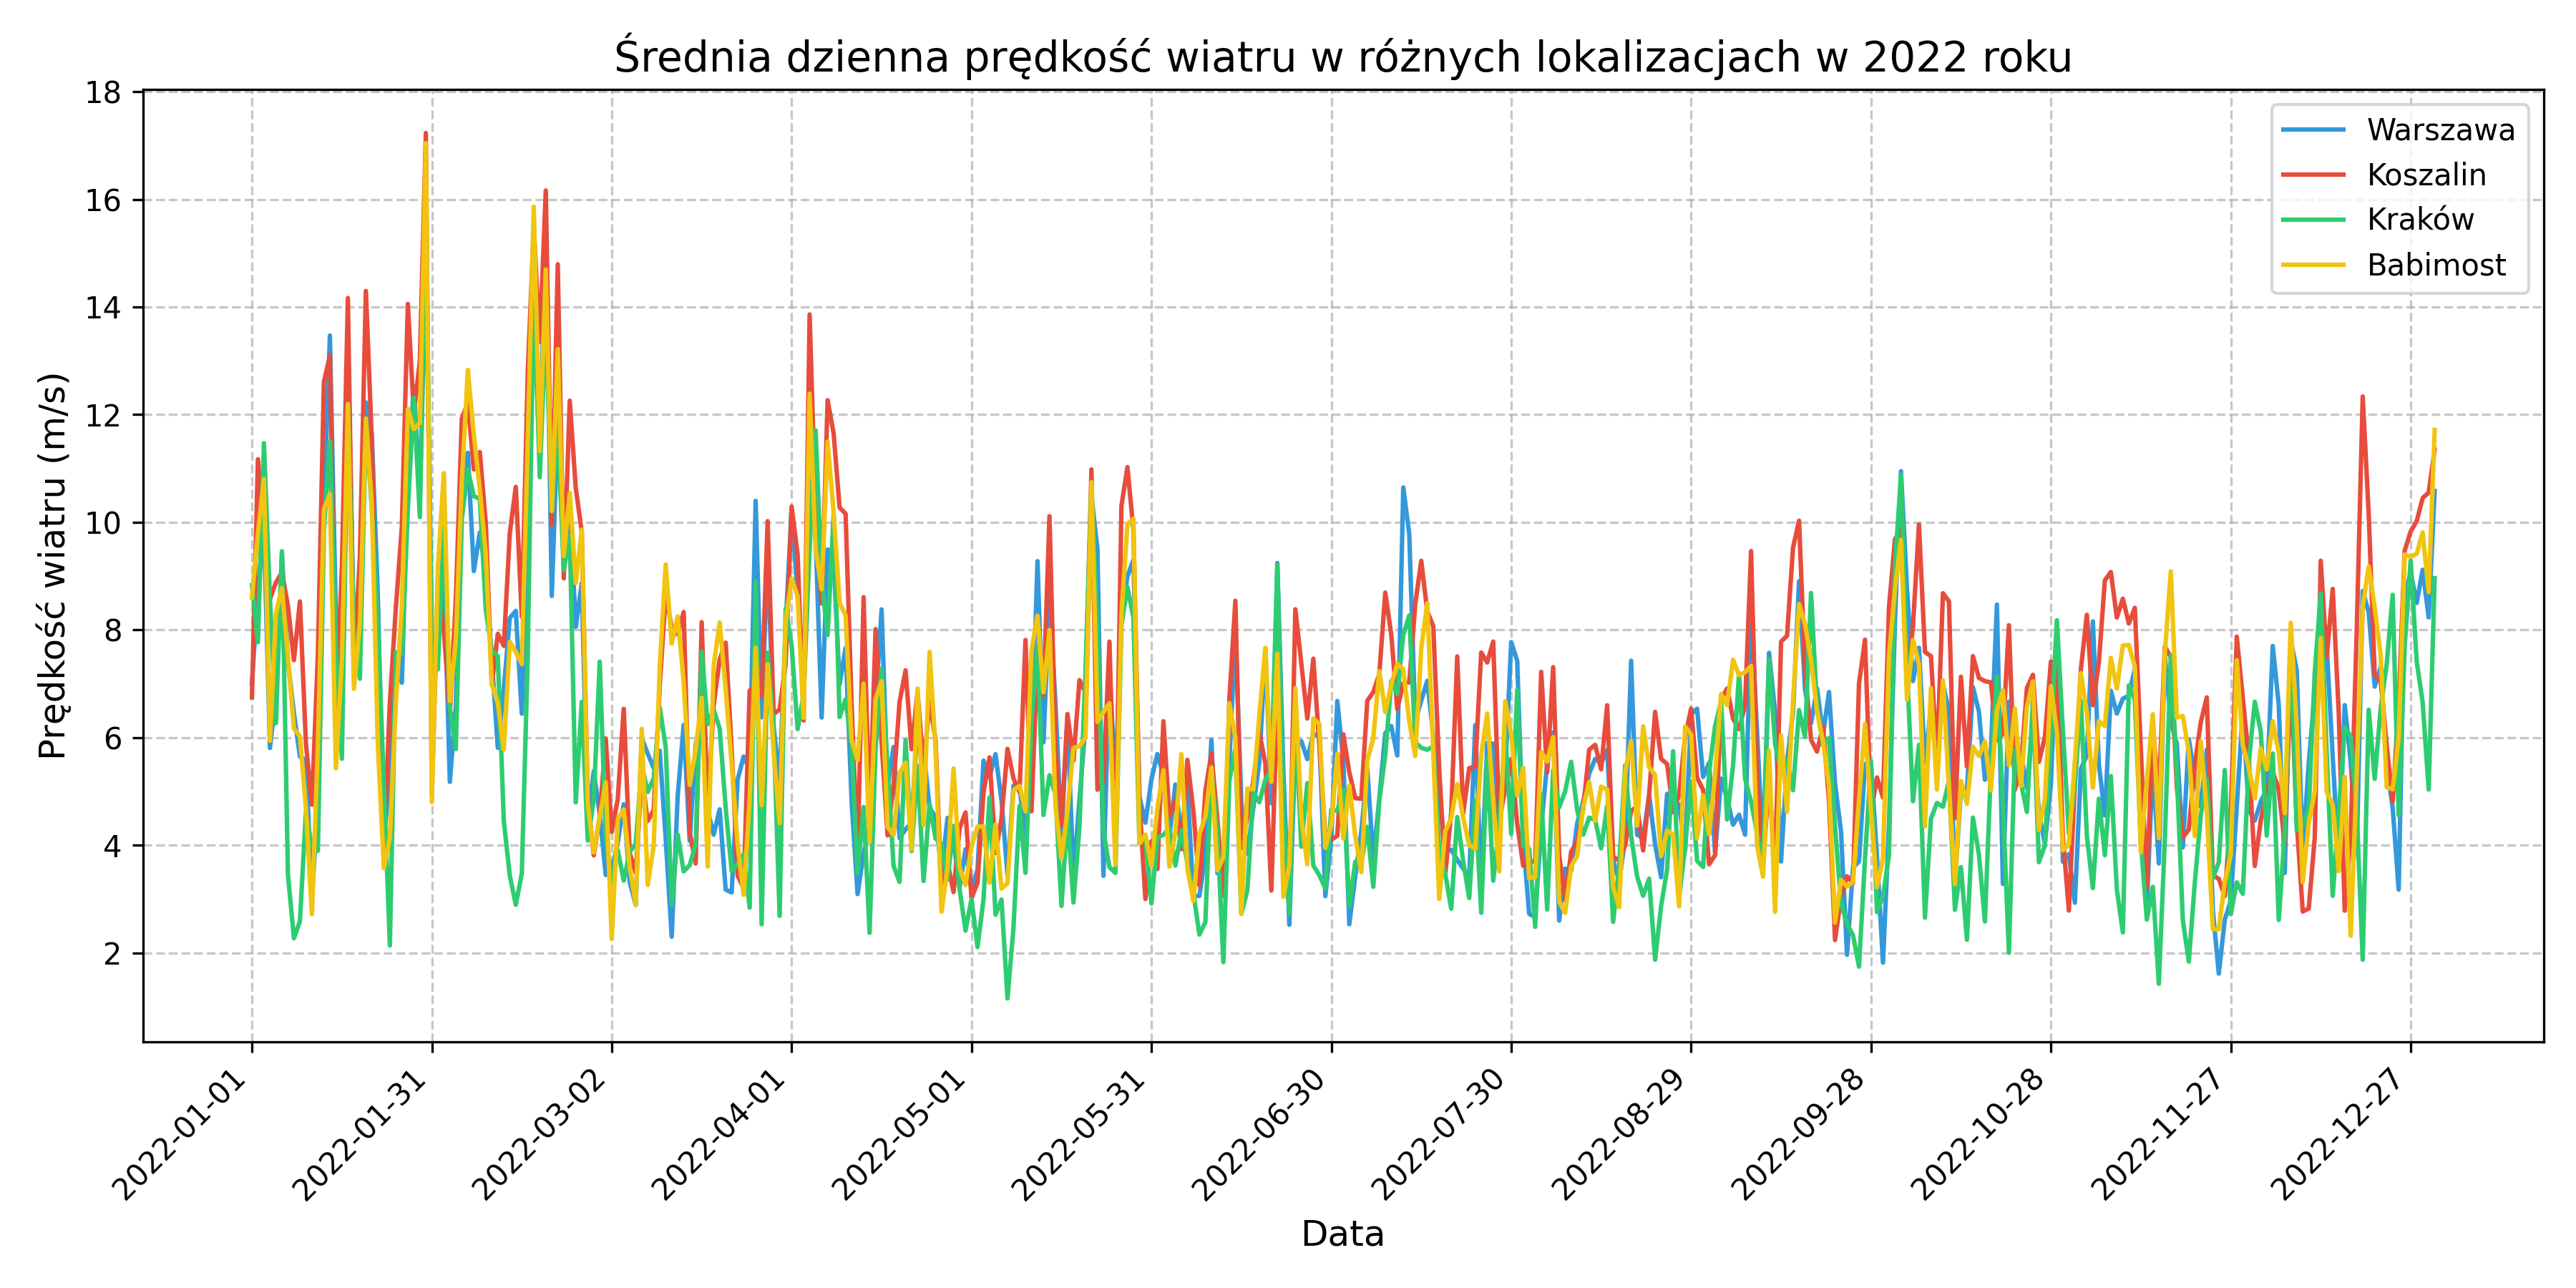
\includegraphics[width=\textwidth]{../plots/weather/wind_speed_time_series_2022.png}
    \caption{Zmienność prędkości wiatru w czasie (2022)}
    \label{fig:wind-speed-time-series-2022}
\end{figure}

\begin{figure}[H]
    \centering
    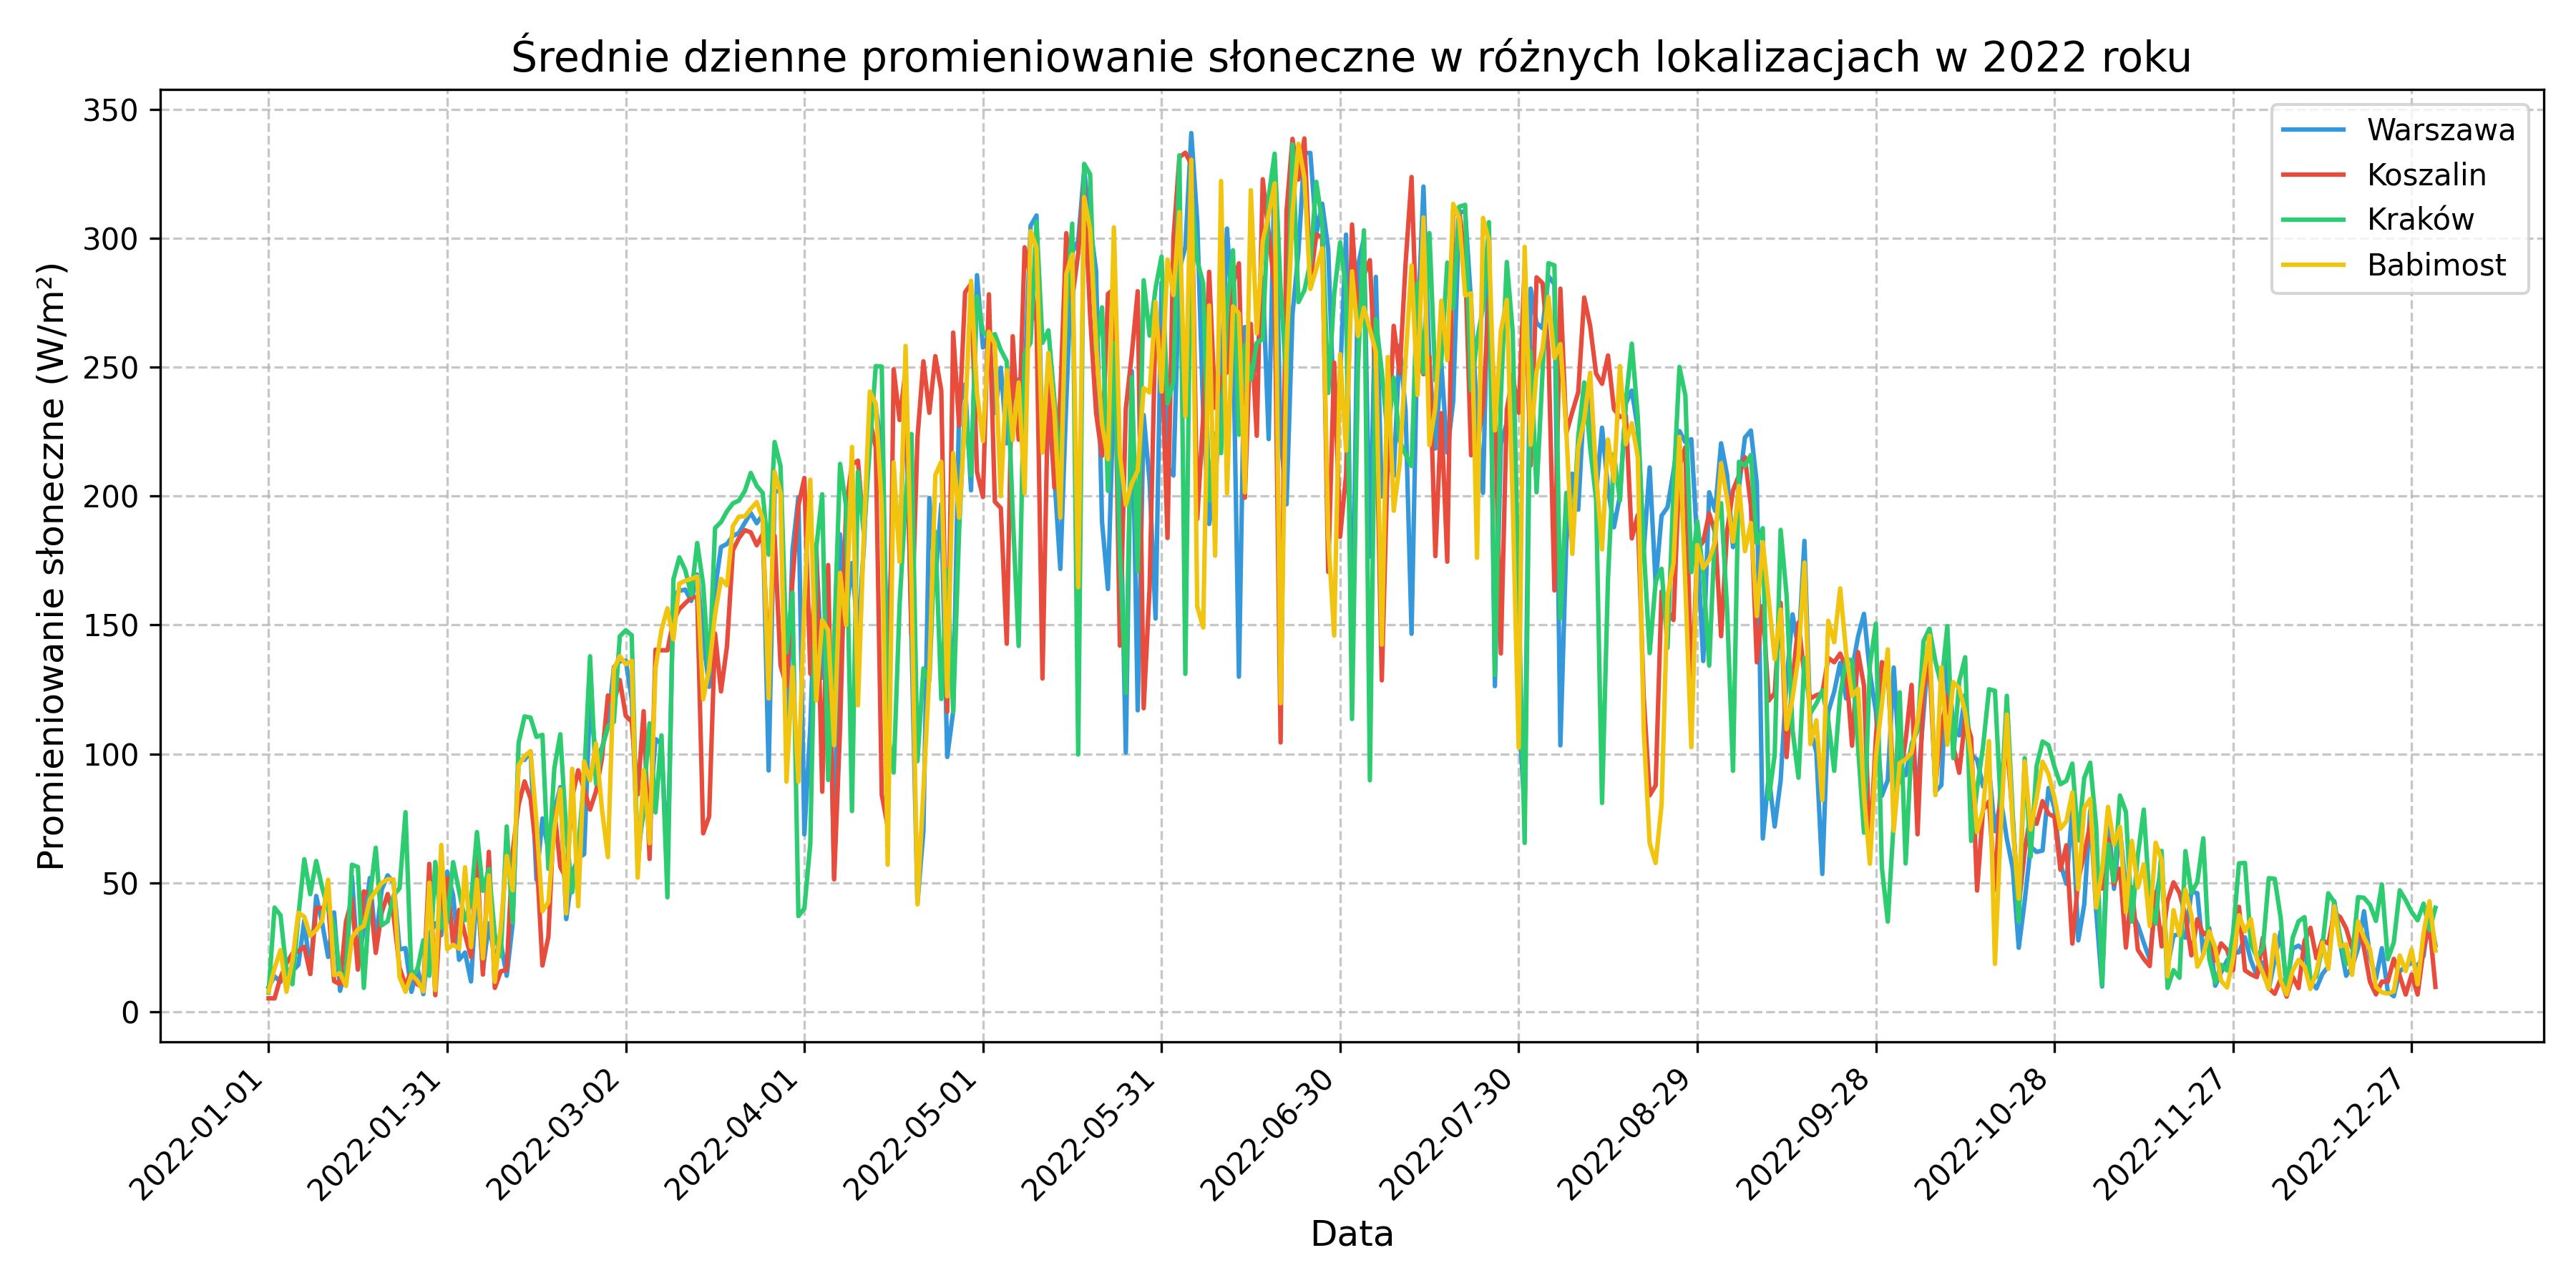
\includegraphics[width=\textwidth]{../plots/weather/solar_radiation_time_series_2022.png}
    \caption{Zmienność promieniowania słonecznego w czasie (2022)}
    \label{fig:solar-radiation-time-series-2022}
\end{figure}

\begin{figure}[H]
    \centering
    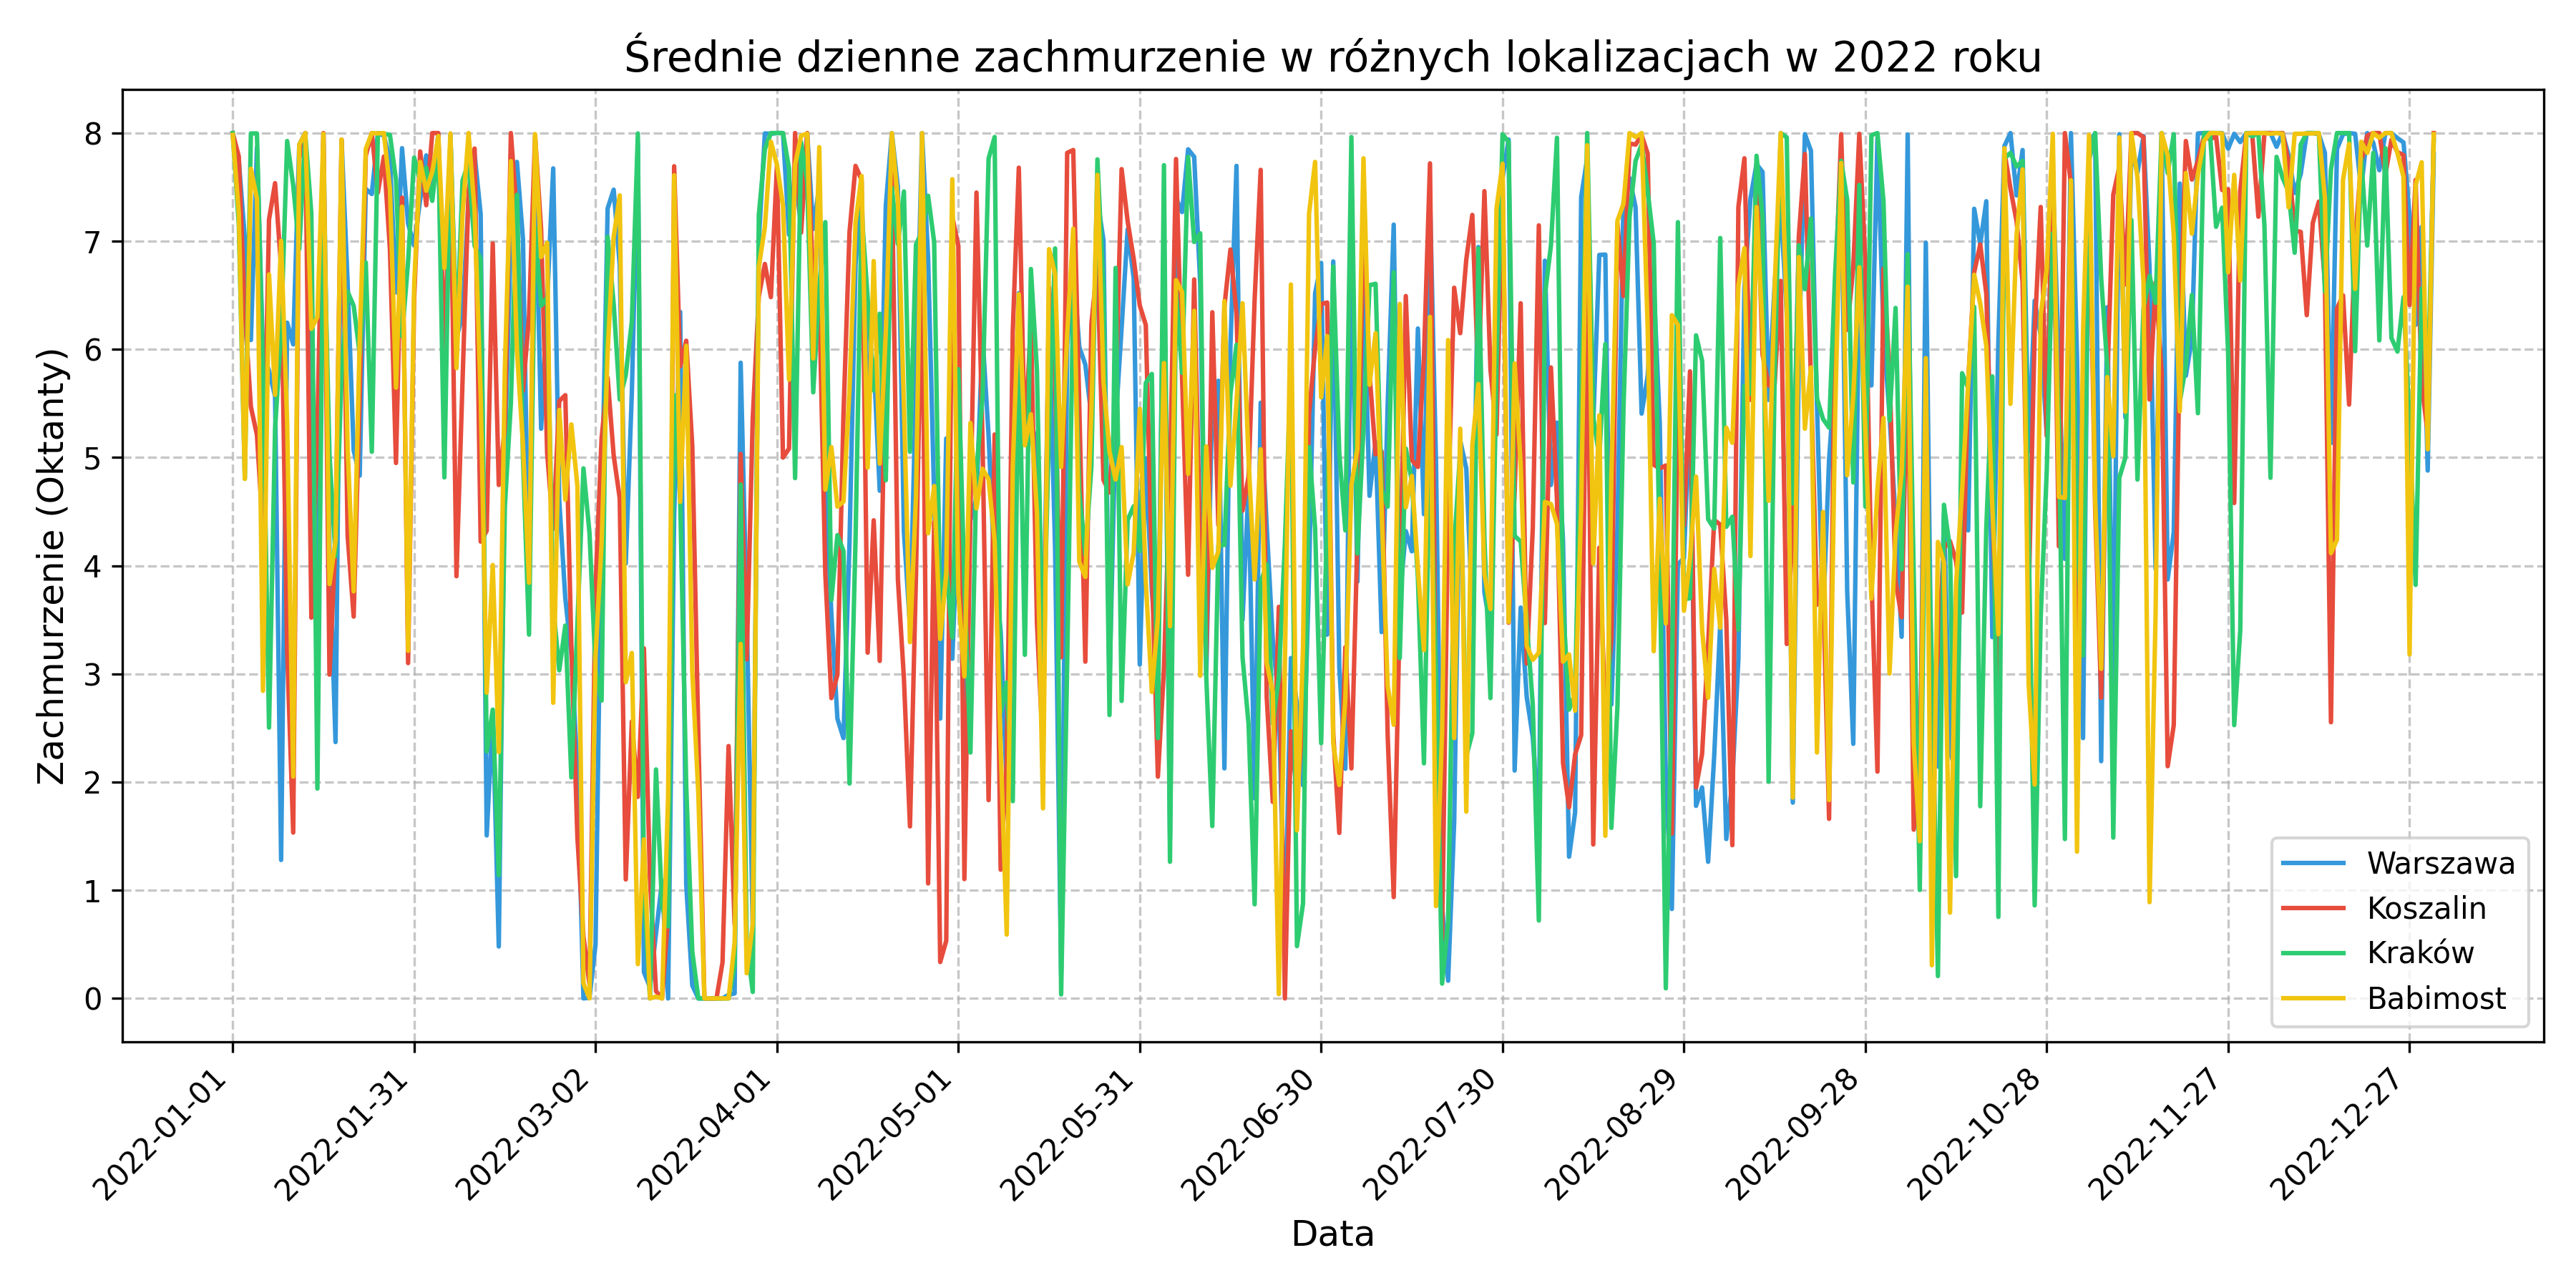
\includegraphics[width=\textwidth]{../plots/weather/cloud_cover_time_series_2022.png}
    \caption{Zmienność zachmurzenia w czasie (2022)}
    \label{fig:cloud-cover-time-series-2022}
\end{figure}

W ramach analizy w późniejszej części pracy spróbuję uprościć model i uśrednić wartości parametrów pogodowych dla całego kraju i sprawdzić czy wynik się poprawi. 

\subsection{Produkcja energii z wybranych źródeł}
Zmienne dotyczące produkcji energii z różnych źródeł odgrywają kluczową rolę w analizie cen energii na Rynku Dnia Następnego (RDN), ponieważ odzwierciedlają strukturę podaży energii w Polsce, która ma bezpośredni wpływ na dynamikę cen. W niniejszej pracy uwzględniono osiem zmiennych opisujących produkcję energii: 
\begin{itemize}
    \item \textbf{hard\_coal} - produkcja z węgla kamiennego (MW),
    \item \textbf{coal\_derived} - produkcja z paliw pochodnych węgla (MW),
    \item \textbf{lignite} - produkcja z węgla brunatnego (MW),
    \item \textbf{gas} - produkcja z gazu ziemnego (MW),
    \item \textbf{oil} - produkcja z ropy naftowej lub jej pochodnych (MW),
    \item \textbf{biomass} - produkcja z biomasy (MW),
    \item \textbf{wind} - produkcja z elektrowni wiatrowych lądowych (MW),
    \item \textbf{solar} - produkcja z paneli fotowoltaicznych (MW).
\end{itemize}

Dane te pochodzą z Polskich Sieci Elektroenergetycznych (PSE) i zostały dopasowane do godzinowego formatu danych RDN, co pozwoliło na ich integrację z pozostałymi zmiennymi. 
\begin{figure}[H]
    \centering
    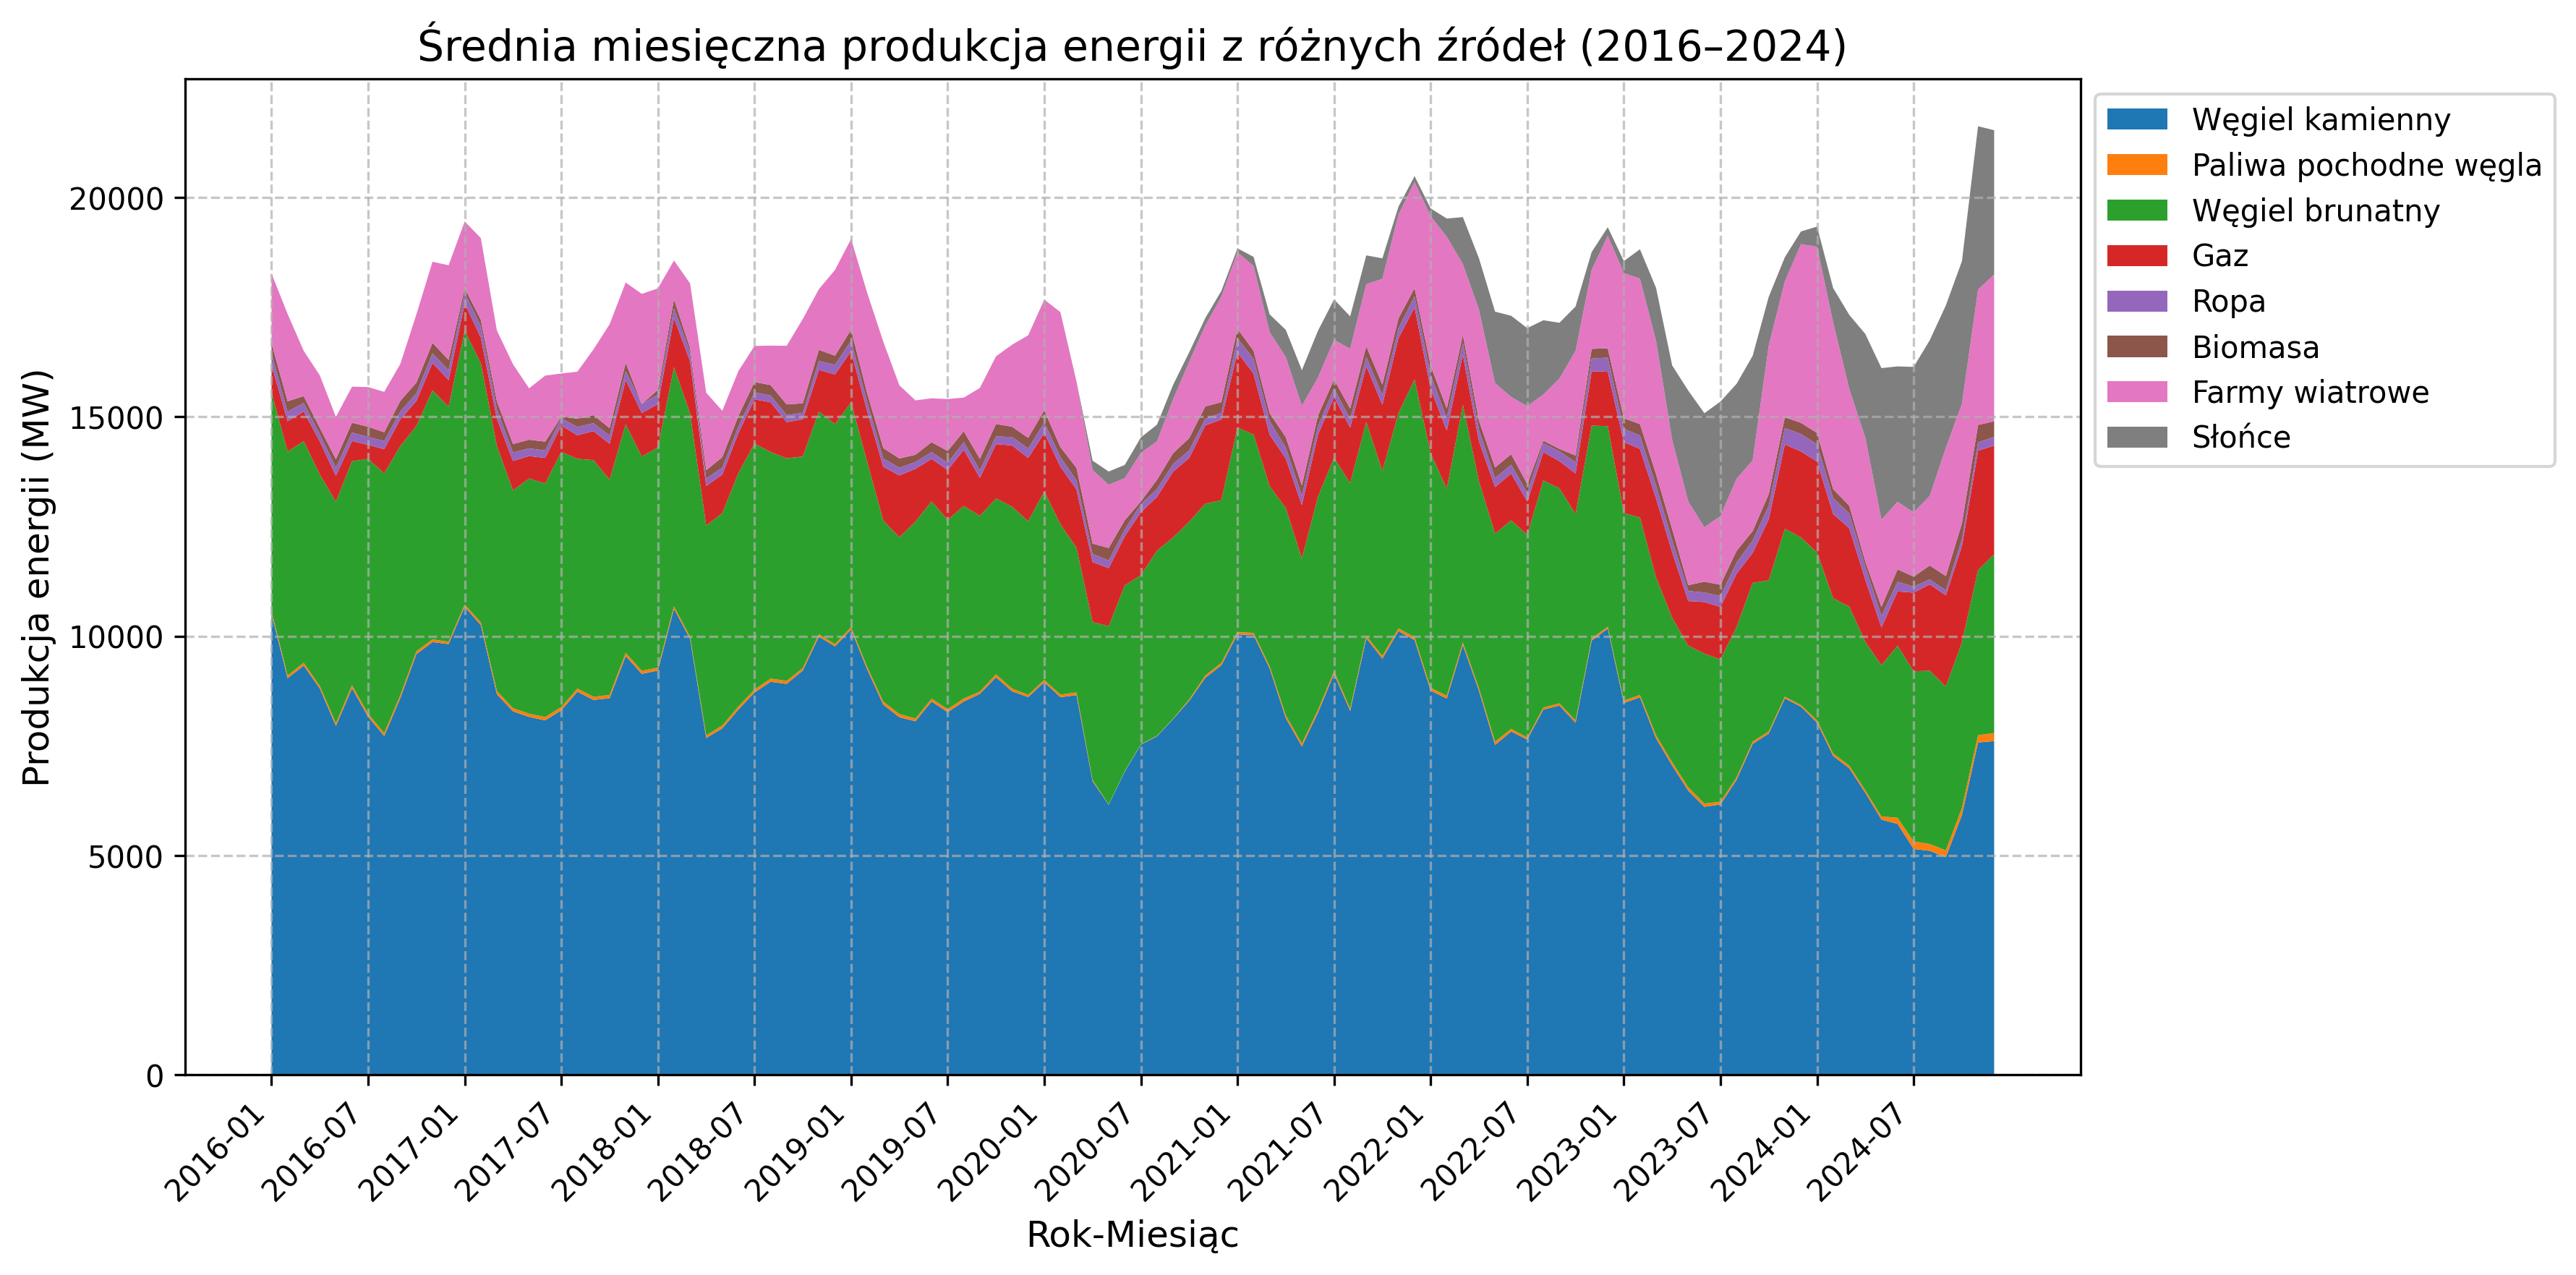
\includegraphics[width=1.0\textwidth]{../plots/energy/energy_production_time_series_full.png}
    \caption{Zmienność produkcji energii z różnych źródeł w czasie (2016–2024)}
    \label{fig:energy-production-time-series-full}
\end{figure}

Wykres powyżej przedstawia średnią miesięczną produkcję energii z różnych źródeł w Polsce w latach 2016–2024, co jest istotne w kontekście prognozowania cen energii (EPF) na Rynku Dnia Następnego (RDN). Wykres obszarowy ukazuje dominację węgla kamiennego i brunatnego, której do tej pory odpowiadają za większość produkcji energii elektrycznej. Biomasa oraz paliwa pochodne węgla stanowią znikomą część podaży i mogą być pominięte dla redukcji ilości zmiennych. Produkcja za pomocą gazu i ropy stale posiada niewielką, ale istotną część produkcji energii. Warto zauważyć, że produkcja z OZE, szczególnie ze słońca znacząco rośnie w ostatnich latach, co może mieć istotny wpływ na ceny energii i umiejętność jej prognozowania. Do poprzednio omówionych zmiennych dodano również zmienną \texttt{non\_emissive\_sources\_percentage}, która reprezentuje procentowy udział energii produkowanej z OZE w całkowitej produkcji energii elektrycznej w Polsce.
\begin{figure}[H]
    \centering
    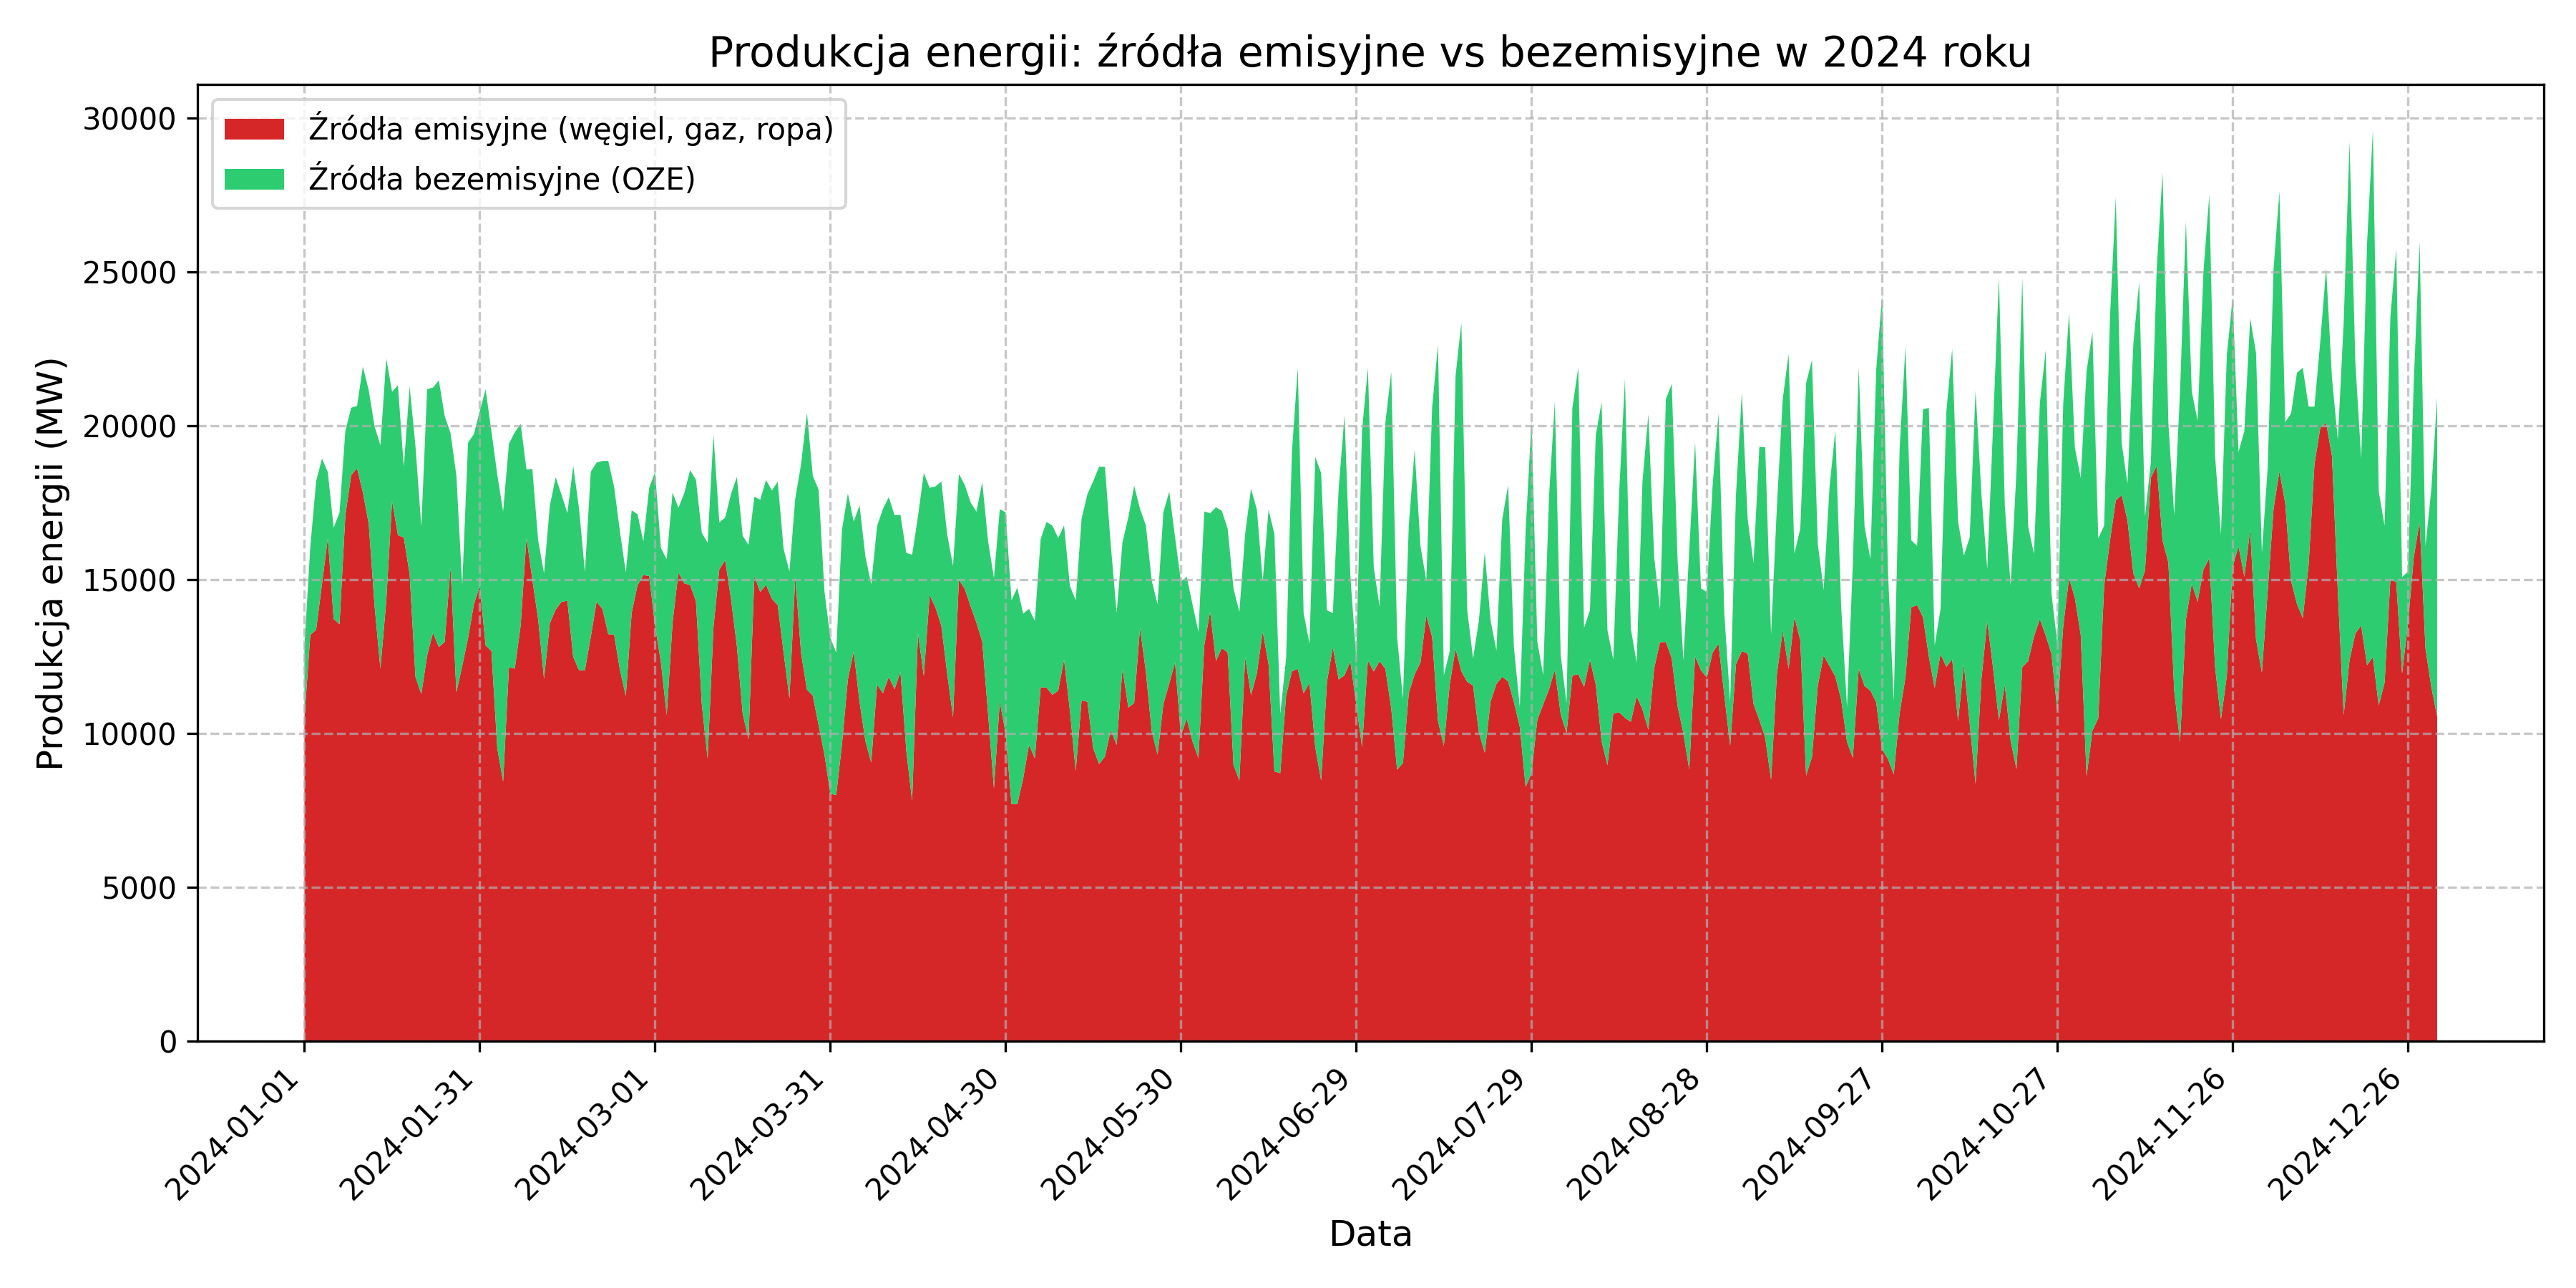
\includegraphics[width=\textwidth]{../plots/energy/emission_vs_non_emission_2024.png}
    \caption{Porównanie produkcji energii z emisyjnych i bezemisyjnych źródeł w 2024 roku}
    \label{fig:emission-vs-non-emission-2024}
\end{figure}
W najbardziej korzystne dla gospodatki momenty część produkcji z OZE może przekraczać zapewnienie energii z węgla, co może prowadzić do spadku cen energii. Warto również zauważyć, że produkcja z węgla kamiennego i brunatnego jest bardziej stabilna i przewidywalna niż produkcja z OZE, co może wpływać na dokładność prognoz. W związku z tym, zmienne dotyczące produkcji energii z różnych źródeł są istotnym elementem analizy i modelowania cen energii na RDN.

\subsection{Handel energią z państwami sąsiednimi}
\label{subsec:trade}
Zmienne dotyczące wymiany energii z innymi krajami są istotnym elementem analizy cen energii na Rynku Dnia Następnego (RDN), ponieważ pozwalają na uwzględnienie wpływu handlu międzynarodowego na ceny energii w Polsce. W niniejszej pracy uwzględnione zostały bilanse handlu energią z Państwami sąsiednimi, z którymi Polska ma połączenia transgraniczne. Są to Państwa takie jak:
\begin{itemize}
    \item Niemcy (DE),
    \item Czechy (CZ),
    \item Słowacja (SK),
    \item Litwa (LT),
    \item Szwecja (SE),
    \item Ukraina (UA).
\end{itemize}

Dane dotyczące wymiany energii z tymi krajami pochodzą z Polskich Sieci Elektroenergetycznych (PSE) i są dostępne w granulacji godzinowej. Warto zauważyć, że Polska jest jednym z kluczowych graczy na rynku energii w Europie Środkowo-Wschodniej, a wymiana energii z innymi krajami może mieć istotny wpływ na ceny energii w Polsce. W szczególności, w okresach wysokiego zapotrzebowania na energię lub w sytuacjach poważnych awarii, Polska może importować energię z innych krajów, co prowadzi do wzrostu cen. Z drugiej strony, w okresach niskiego zapotrzebowania, Polska może eksportować, czyli sprzedawać nadwyżki energii, co może prowadzić do spadku cen. Poniżej przedstawiam wykresy dotyczące wymiany energii z sąsiadami w latach 2016-2024.

\begin{table}[H]
    \centering
    \resizebox{\textwidth}{!}{%
    \begin{tabular}{|c|r|r|r|r|r|r|}
    \hline
    \textbf{Rok} & \textbf{Niemcy (MW)} & \textbf{Czechy (MW)} & \textbf{Litwa (MW)} & \textbf{Słowacja (MW)} & \textbf{Szwecja (MW)} & \textbf{Ukraina (MW)} \\ \hline
    2016 & 994.26  & -761.81 & 68.21   & -475.47 & 294.36  & 108.99  \\ \hline
    2017 & 836.24  & -612.73 & 119.92  & -499.21 & 340.96  & 102.45  \\ \hline
    2018 & 803.00  & -373.78 & 102.53  & -366.14 & 310.83  & 160.96  \\ \hline
    2019 & 1149.22 & -312.31 & 216.38  & -367.32 & 329.80  & 157.17  \\ \hline
    2020 & 1275.75 & -264.90 & 201.93  & -348.95 & 428.81  & 167.98  \\ \hline
    2021 & 957.79  & -901.92 & 110.04  & -519.59 & 364.69  & 93.55   \\ \hline
    2022 & 918.62  & -1000.89 & 86.53  & -684.25 & 429.17  & 126.95  \\ \hline
    2023 & 851.27  & -526.46 & 58.40   & -382.18 & 431.60  & 5.76    \\ \hline
    2024 & 1005.26 & -544.15 & -112.90 & -389.65 & 296.29  & -68.03  \\ \hline
    \end{tabular}%
    }
    \caption{Średni bilans wymiany energii z sąsiadami w latach 2016–2024}
    \label{tab:energy-trade-balance}
\end{table}

Wartości te są średniogodzinowymi bilansami wymiany energii z sąsiadami w latach 2016-2024. Wartości dodatnie oznaczają eksport energii, a wartości ujemne import energii. Polska ma dodatni bilans wymiany energii z Niemcami, co oznacza, że Polska regularnie eksportuje energię do Niemiec. Największe ujemne bilanse Polska posiada z Czechami, prawdopodobnie spowodowane jest to funkcjonującymi w Czechami elektrowniami atomowymi. Te przepływy wpływają na ceny na RDN: eksport do Niemiec i Szwecji może podnosić ceny w Polsce, a import z Czech i Słowacji stabilizuje system, ale zwiększa zależność od zewnętrznych dostawców.

\subsection{Ceny paliw kopalnych i emisji CO2}
\label{subsec:prices}

Zmienne dotyczące cen paliw kopalnych oraz emisji CO$_2$ odgrywają kluczową rolę w analizie cen energii na Rynku Dnia Następnego (RDN), ponieważ koszty paliw i emisji mają bezpośredni wpływ na ceny energii elektrycznej w Polsce, gdzie dominującym źródłem energii jest węgiel. W niniejszej pracy uwzględniono cztery zmienne, które zostały opisane w Tabeli~\ref{tab:fuel_variables}.

\begin{table}[H]
    \centering
    \begin{tabular}{|l|l|l|l|}
    \hline
    \textbf{Nazwa zmiennej} & \textbf{Opis} & \textbf{Źródło danych} & \textbf{Granulacja} \\ \hline
    \texttt{gas\_price}     & Cena gazu ziemnego (PLN/MWh) & energy.instrat.pl & Dzienna \\ \hline
    \texttt{coal\_price}    & Cena węgla kamiennego (PLN/GJ) & energy.instrat.pl & miesięczna \\ \hline
    \texttt{co2\_price}     & Cena uprawnień do emisji CO$_2$ (PLN/tCO$_2$) & energy.instrat.pl & tygodniowa \\ \hline
    \texttt{brent\_price}   & Cena ropy Brent Europe (PLN/bar) & www.eia.gov & Dzienna \\ \hline
    \end{tabular}
    \caption{Opis zmiennych dotyczących cen paliw kopalnych i emisji CO$_2$.}
    \label{tab:fuel_variables}
\end{table}

Dane te zostały dopasowane do godzinowego formatu danych RDN, w taki sposób, że w dniach pracy giełdy i znanych cen paliw, cena stale jest przypisana do godzin, a w dniach wolnych od pracy lub bez znanych cen, wartości są interpolowane. 

Ceny paliw kopalnych i emisji CO$_2$ są istotne w kontekście prognozowania cen energii, ponieważ wpływają na koszty produkcji energii w elektrowniach konwencjonalnych, które dominują w polskim miksie energetycznym. Na przykład, wzrost ceny węgla (\texttt{coal\_price}) lub uprawnień do emisji CO$_2$ (\texttt{co2\_price}) zwiększa koszty produkcji energii w elektrowniach węglowych. Cena gazu (\texttt{gas\_price}) jest kluczowa dla elektrowni gazowych, które pełnią rolę bilansującą w systemie. Cena ropy Brent (\texttt{brent\_price}) ma mniejszy bezpośredni wpływ na produkcję energii w Polsce, ale jest istotna w kontekście globalnych trendów cen paliw, które mogą wpływać na inne zmienne, takie jak cena gazu.

Aby zilustrować dynamikę tych zmiennych, na rysunku poniżej przedstawiono zmiany cen paliw kopalnych i emisji CO$_2$ w latach 2016-2024 w ujęciu miesięcznym. Dla lepszego przedstawienia danych użyłem skali logarytmicznej.

\begin{figure}[h]
    \centering
    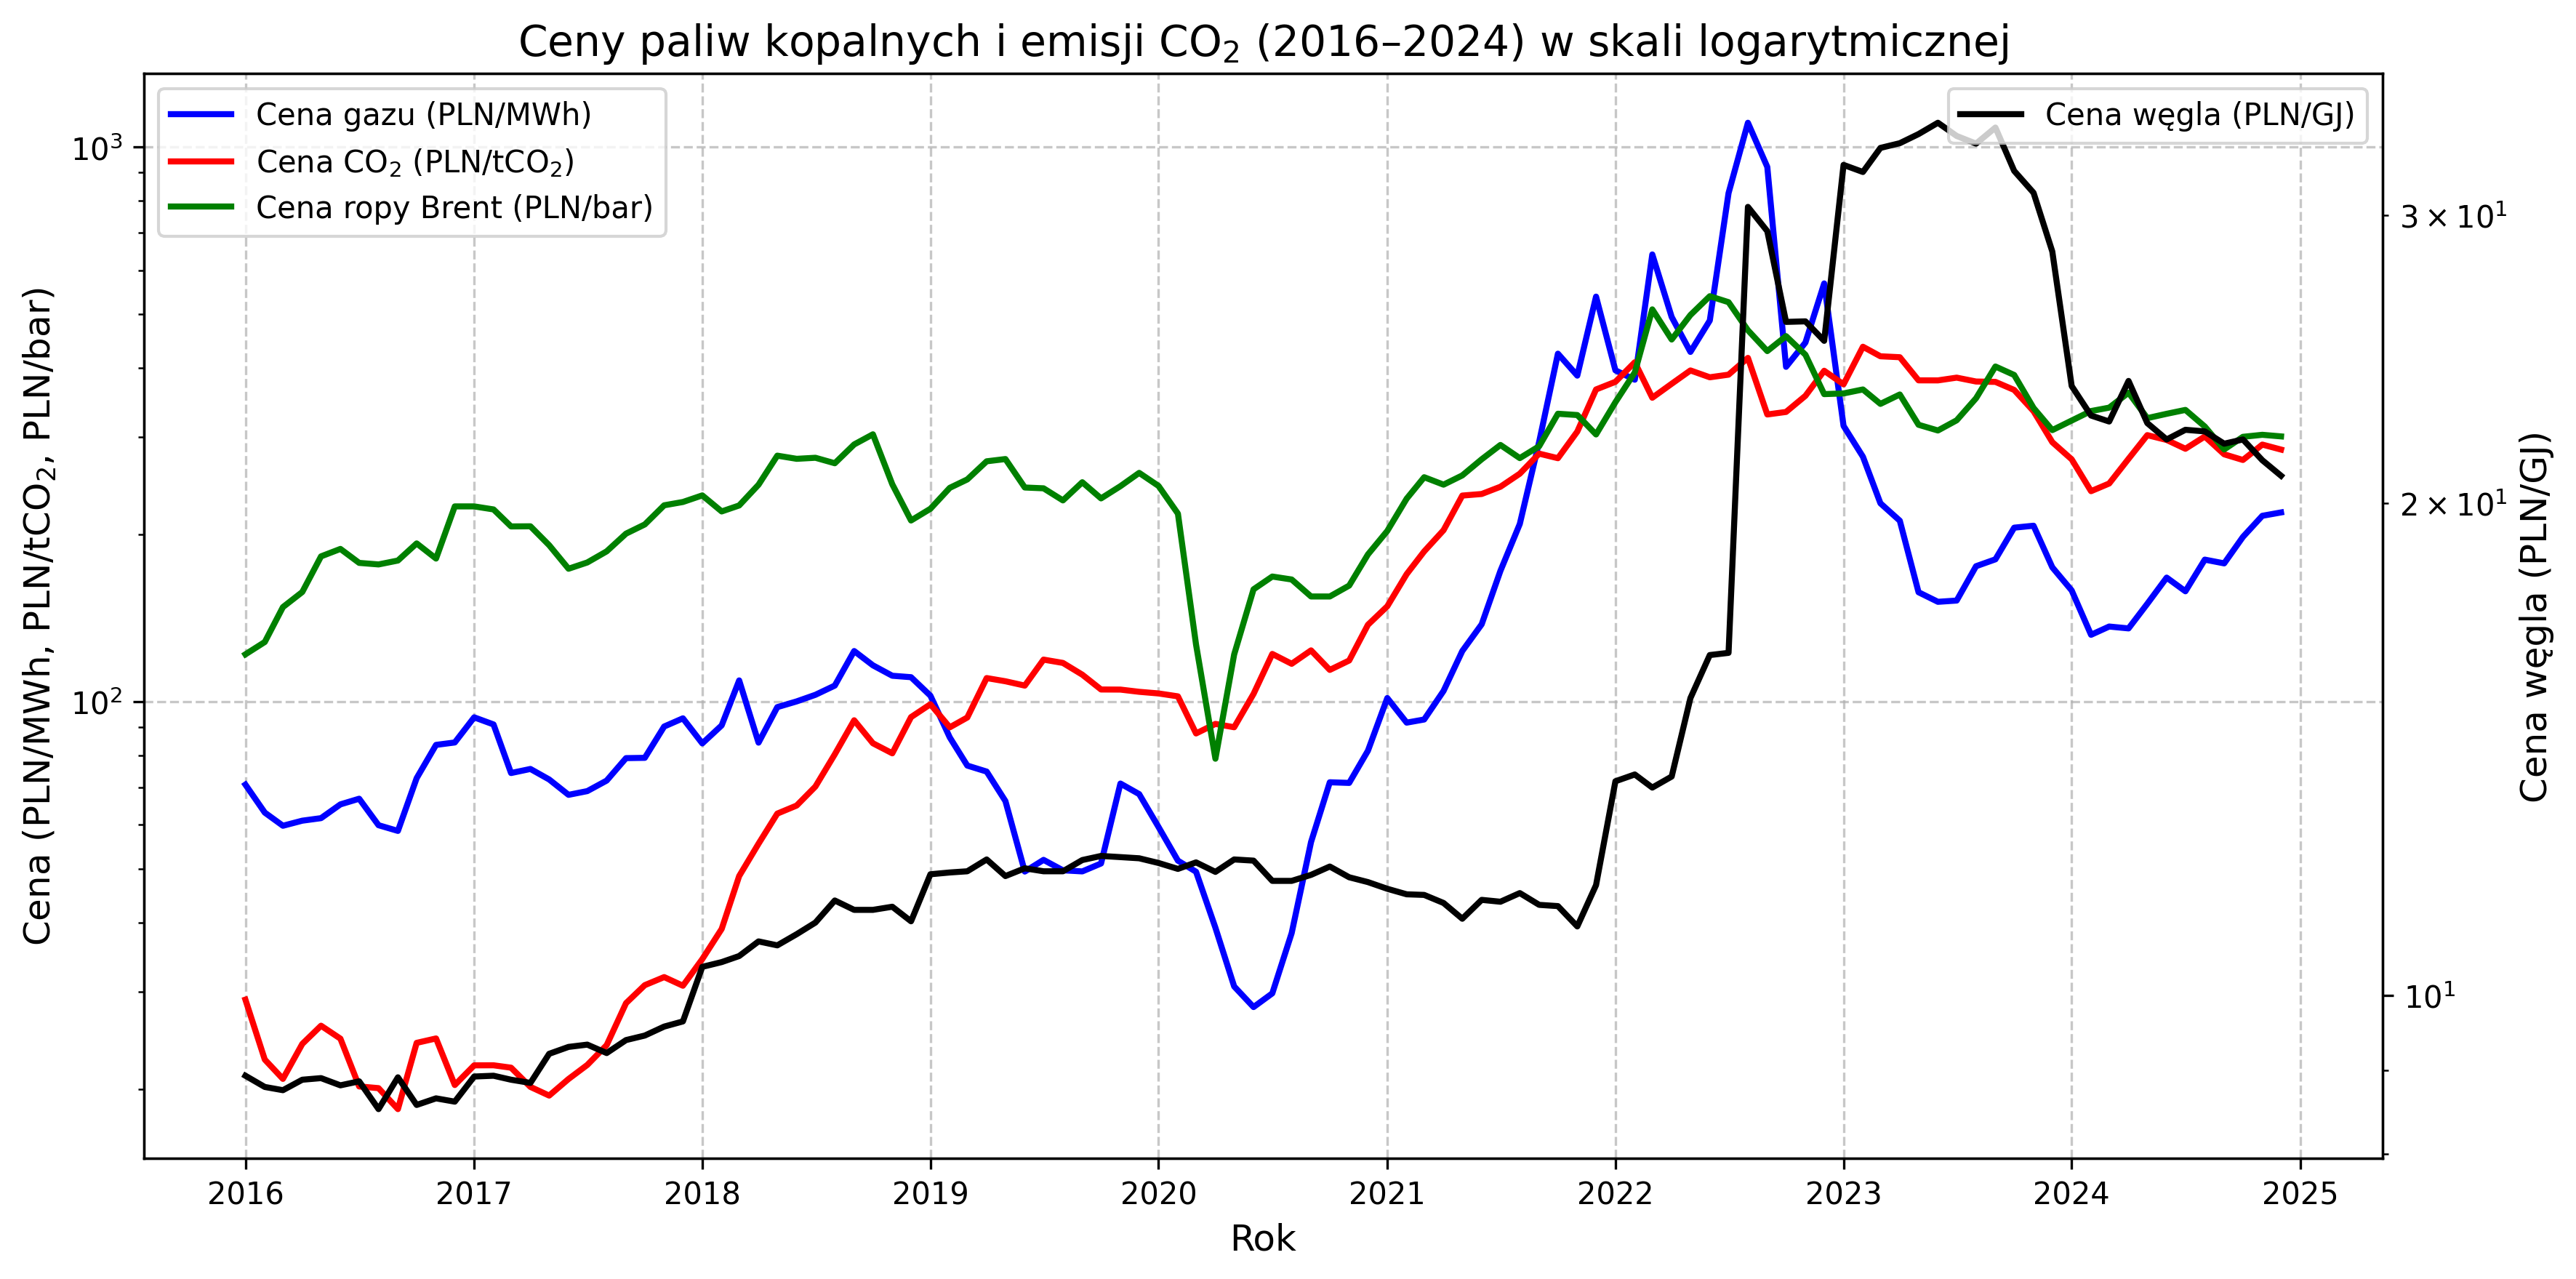
\includegraphics[width=0.9\textwidth]{../plots/fuels/fuel_prices_2016_2024.png}
    \caption{Ceny paliw kopalnych i emisji CO$_2$ w latach 2016-2024 (w ujęciu miesięcznym). Źródło: Opracowanie własne na podstawie danych rynkowych.}
    \label{fig:fuel_prices}
\end{figure}

Ceny paliw kopalnych w okresie wysokiej zmienności szybko rosną, co prawdopodobnie jest przyczyną rosnących cen energii. Największy wzrost ma cena gazu, która od rozpoczęcia konfliktu zbrojnego wzrosła ponad 10-krotnie w ciągu roku. 

\subsection{Straty mocy w systemie elektroenergetycznym}
\label{subsec:losses}

Zmienne dotyczące strat mocy w systemie elektroenergetycznym odgrywają istotną rolę w analizie cen energii na Rynku Dnia Następnego (RDN), ponieważ wpływają na dostępność energii w systemie oraz koszty jej przesyłu i dystrybucji. W niniejszej pracy uwzględniono następujące dane zbierane przez systemy PSE: \texttt{power\_loss} (utrata mocy w wyniku awarii w MW) oraz \texttt{network\_loss} (utrata mocy w sieci w MW). Udostępnione dane mają granulację godzinową. 

Straty mocy w systemie elektroenergetycznym są kluczowe w kontekście prognozowania cen energii, ponieważ zmniejszają ilość energii dostępnej dla odbiorców, co może prowadzić do wzrostu cen na RDN oraz \gls{rb}. Utrata mocy w wyniku awarii

Aby zilustrować dynamikę tych zmiennych, na rysunku~\ref{fig:power_losses} przedstawiono zmiany strat mocy w wyniku awarii (\texttt{power\_loss}) oraz strat mocy w sieci (\texttt{network\_loss}) w latach 2016-2024 w ujęciu miesięcznym.

\begin{figure}[h]
    \centering
    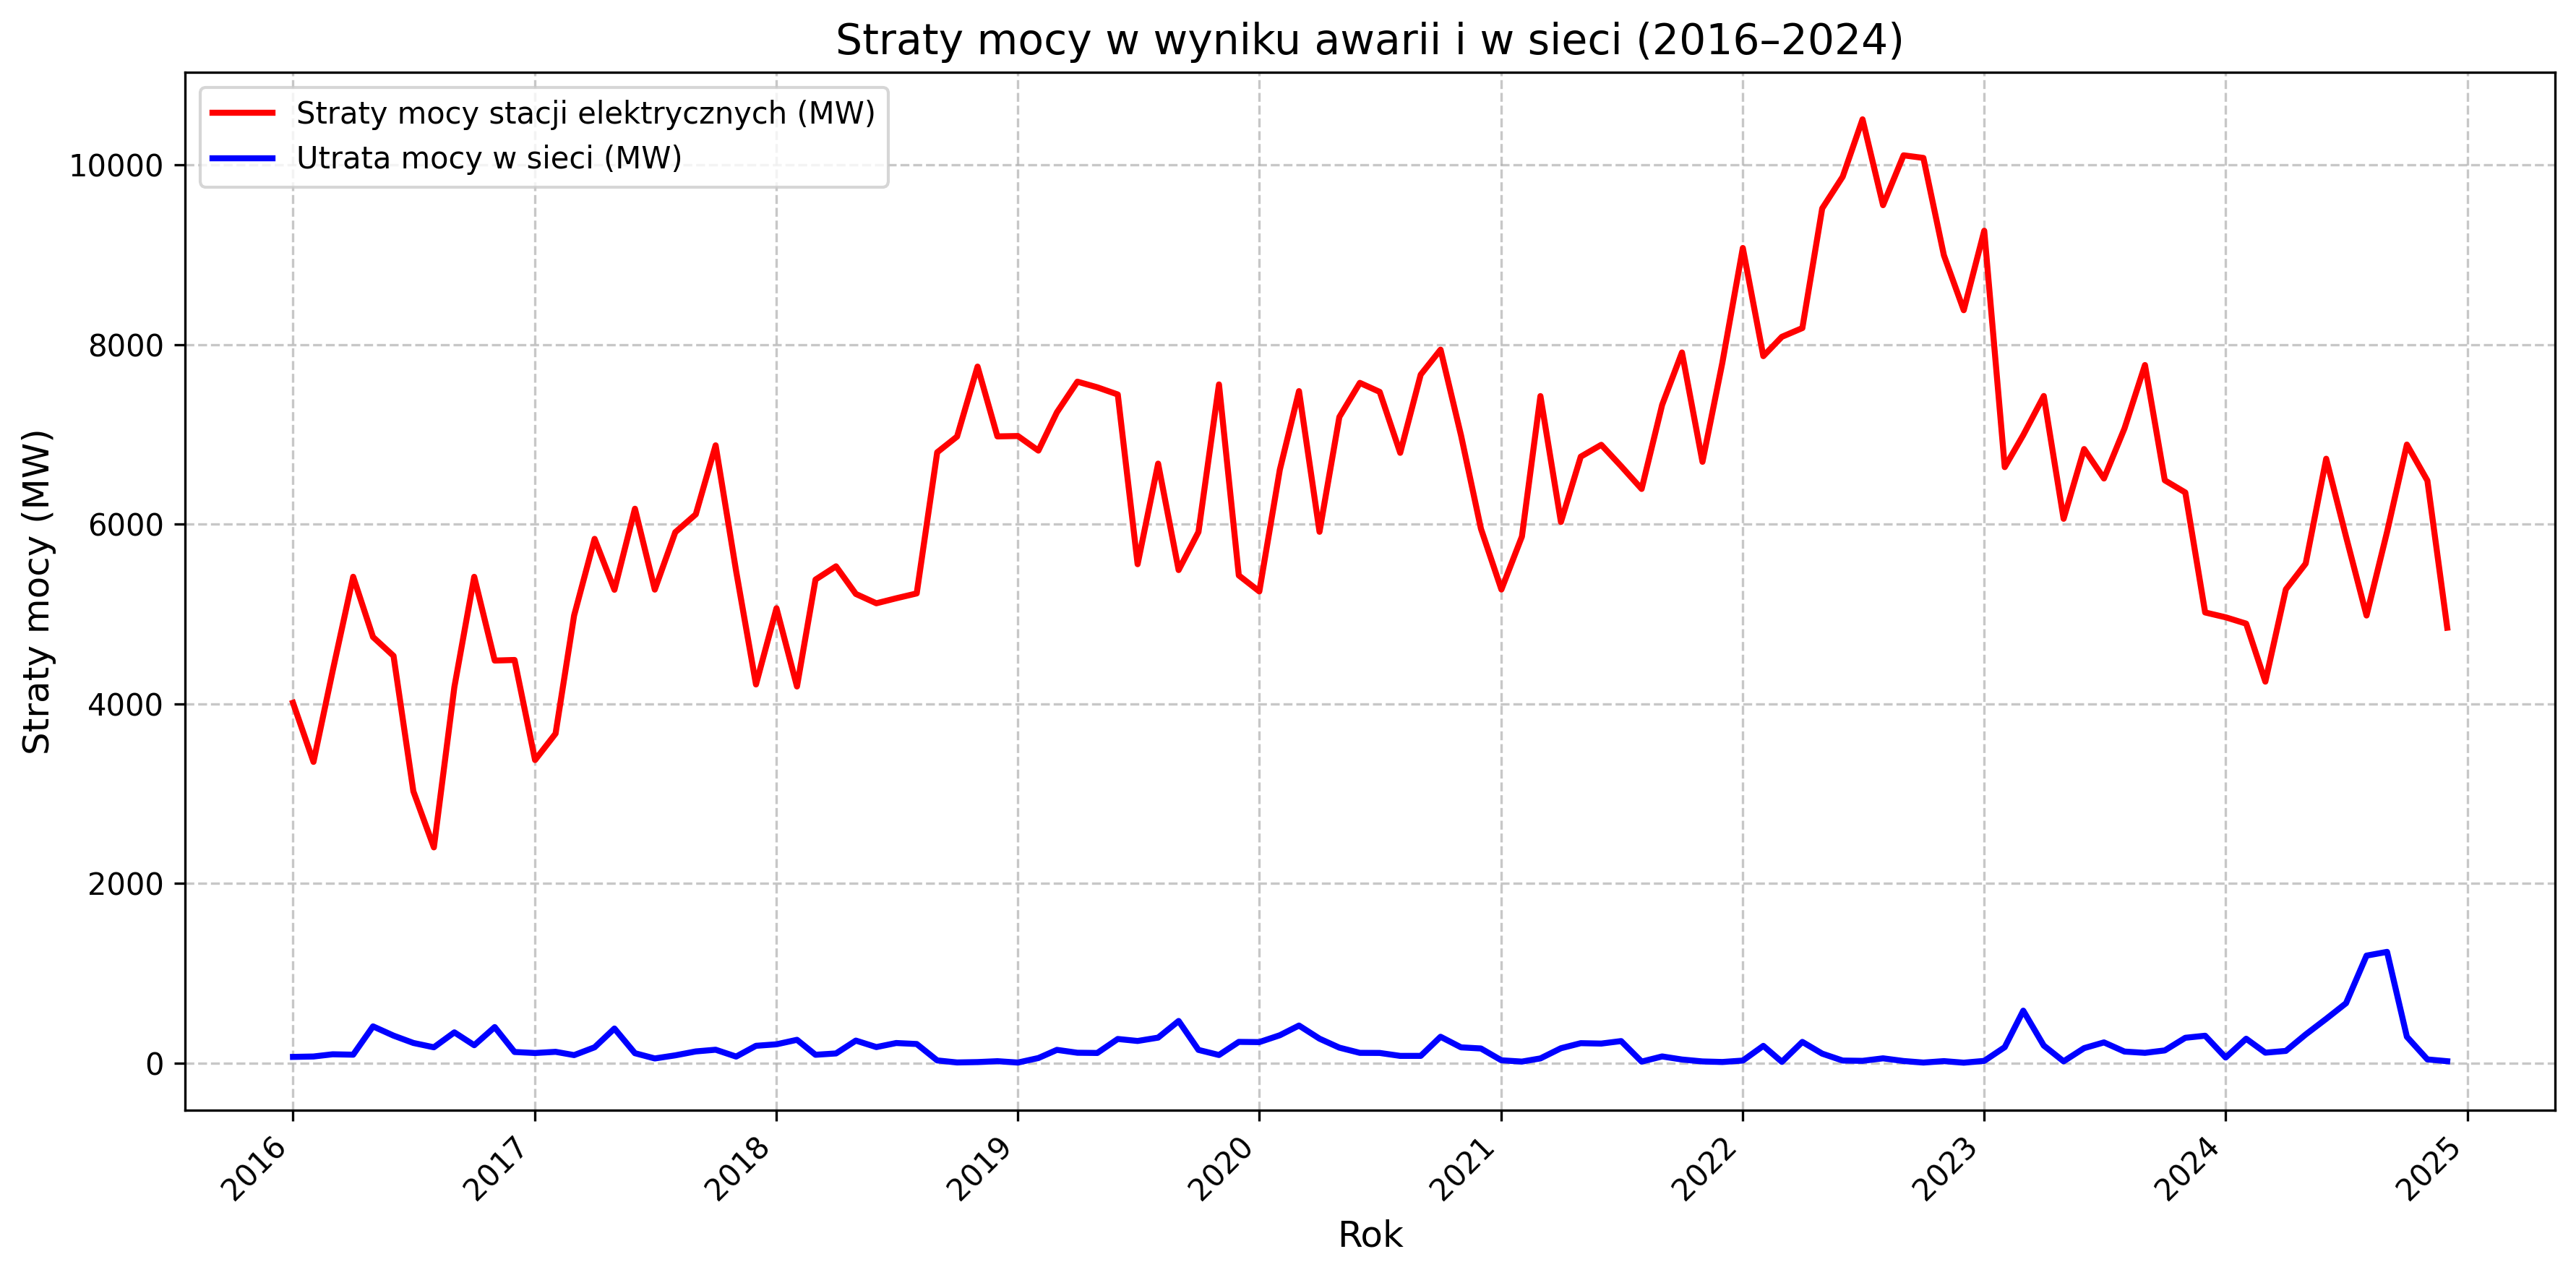
\includegraphics[width=0.9\textwidth]{../plots/losses/power_losses_2016_2024.png}
    \caption{Straty mocy w wyniku awarii i w sieci w latach 2016-2024 (w ujęciu miesięcznym). Źródło: Opracowanie własne na podstawie danych z PSE.}
    \label{fig:power_losses}
\end{figure}

Straty sieciowe na wykresie po 06.2024 są większe od poprzednich. Wynika to ze zmiany metodyki obliczania strat sieciowych przez PSE. Niemniej jednak straty mocy są znaczące, ale wynikają prawdopodbnie z tego, że nie wszystkie jednostki wytworcze pracują w danym momencie lub z ograniczonej ich eksploatacji. 

\subsection{Zapotrzebowanie na energię i wolumen handlu}
\label{subsec:demand}

Zmienne dotyczące zapotrzebowania na energię i wolumenu handlu są kluczowe w analizie cen energii na Rynku Dnia Następnego (RDN), ponieważ mają bezpośredni wpływ na równowagę między podażą a popytem, co jest podstawowym czynnikiem kształtującym ceny energii. W niniejszej pracy uwzględniono następujące zmienne: \texttt{load} (zapotrzebowanie na energię w MWh) oraz \texttt{trade\_volume} (wolumen handlu w MWh). Obie zmienne pochodzą z Polskich Sieci Elektroenergetycznych (PSE) i są dostępne w granulacji godzinowej.

Poniżej na wspólnym wykresie przedstawię różnice pomiędzy zapotrzebowaniem a wolumenem handlu.

\begin{figure}[H]
    \centering
    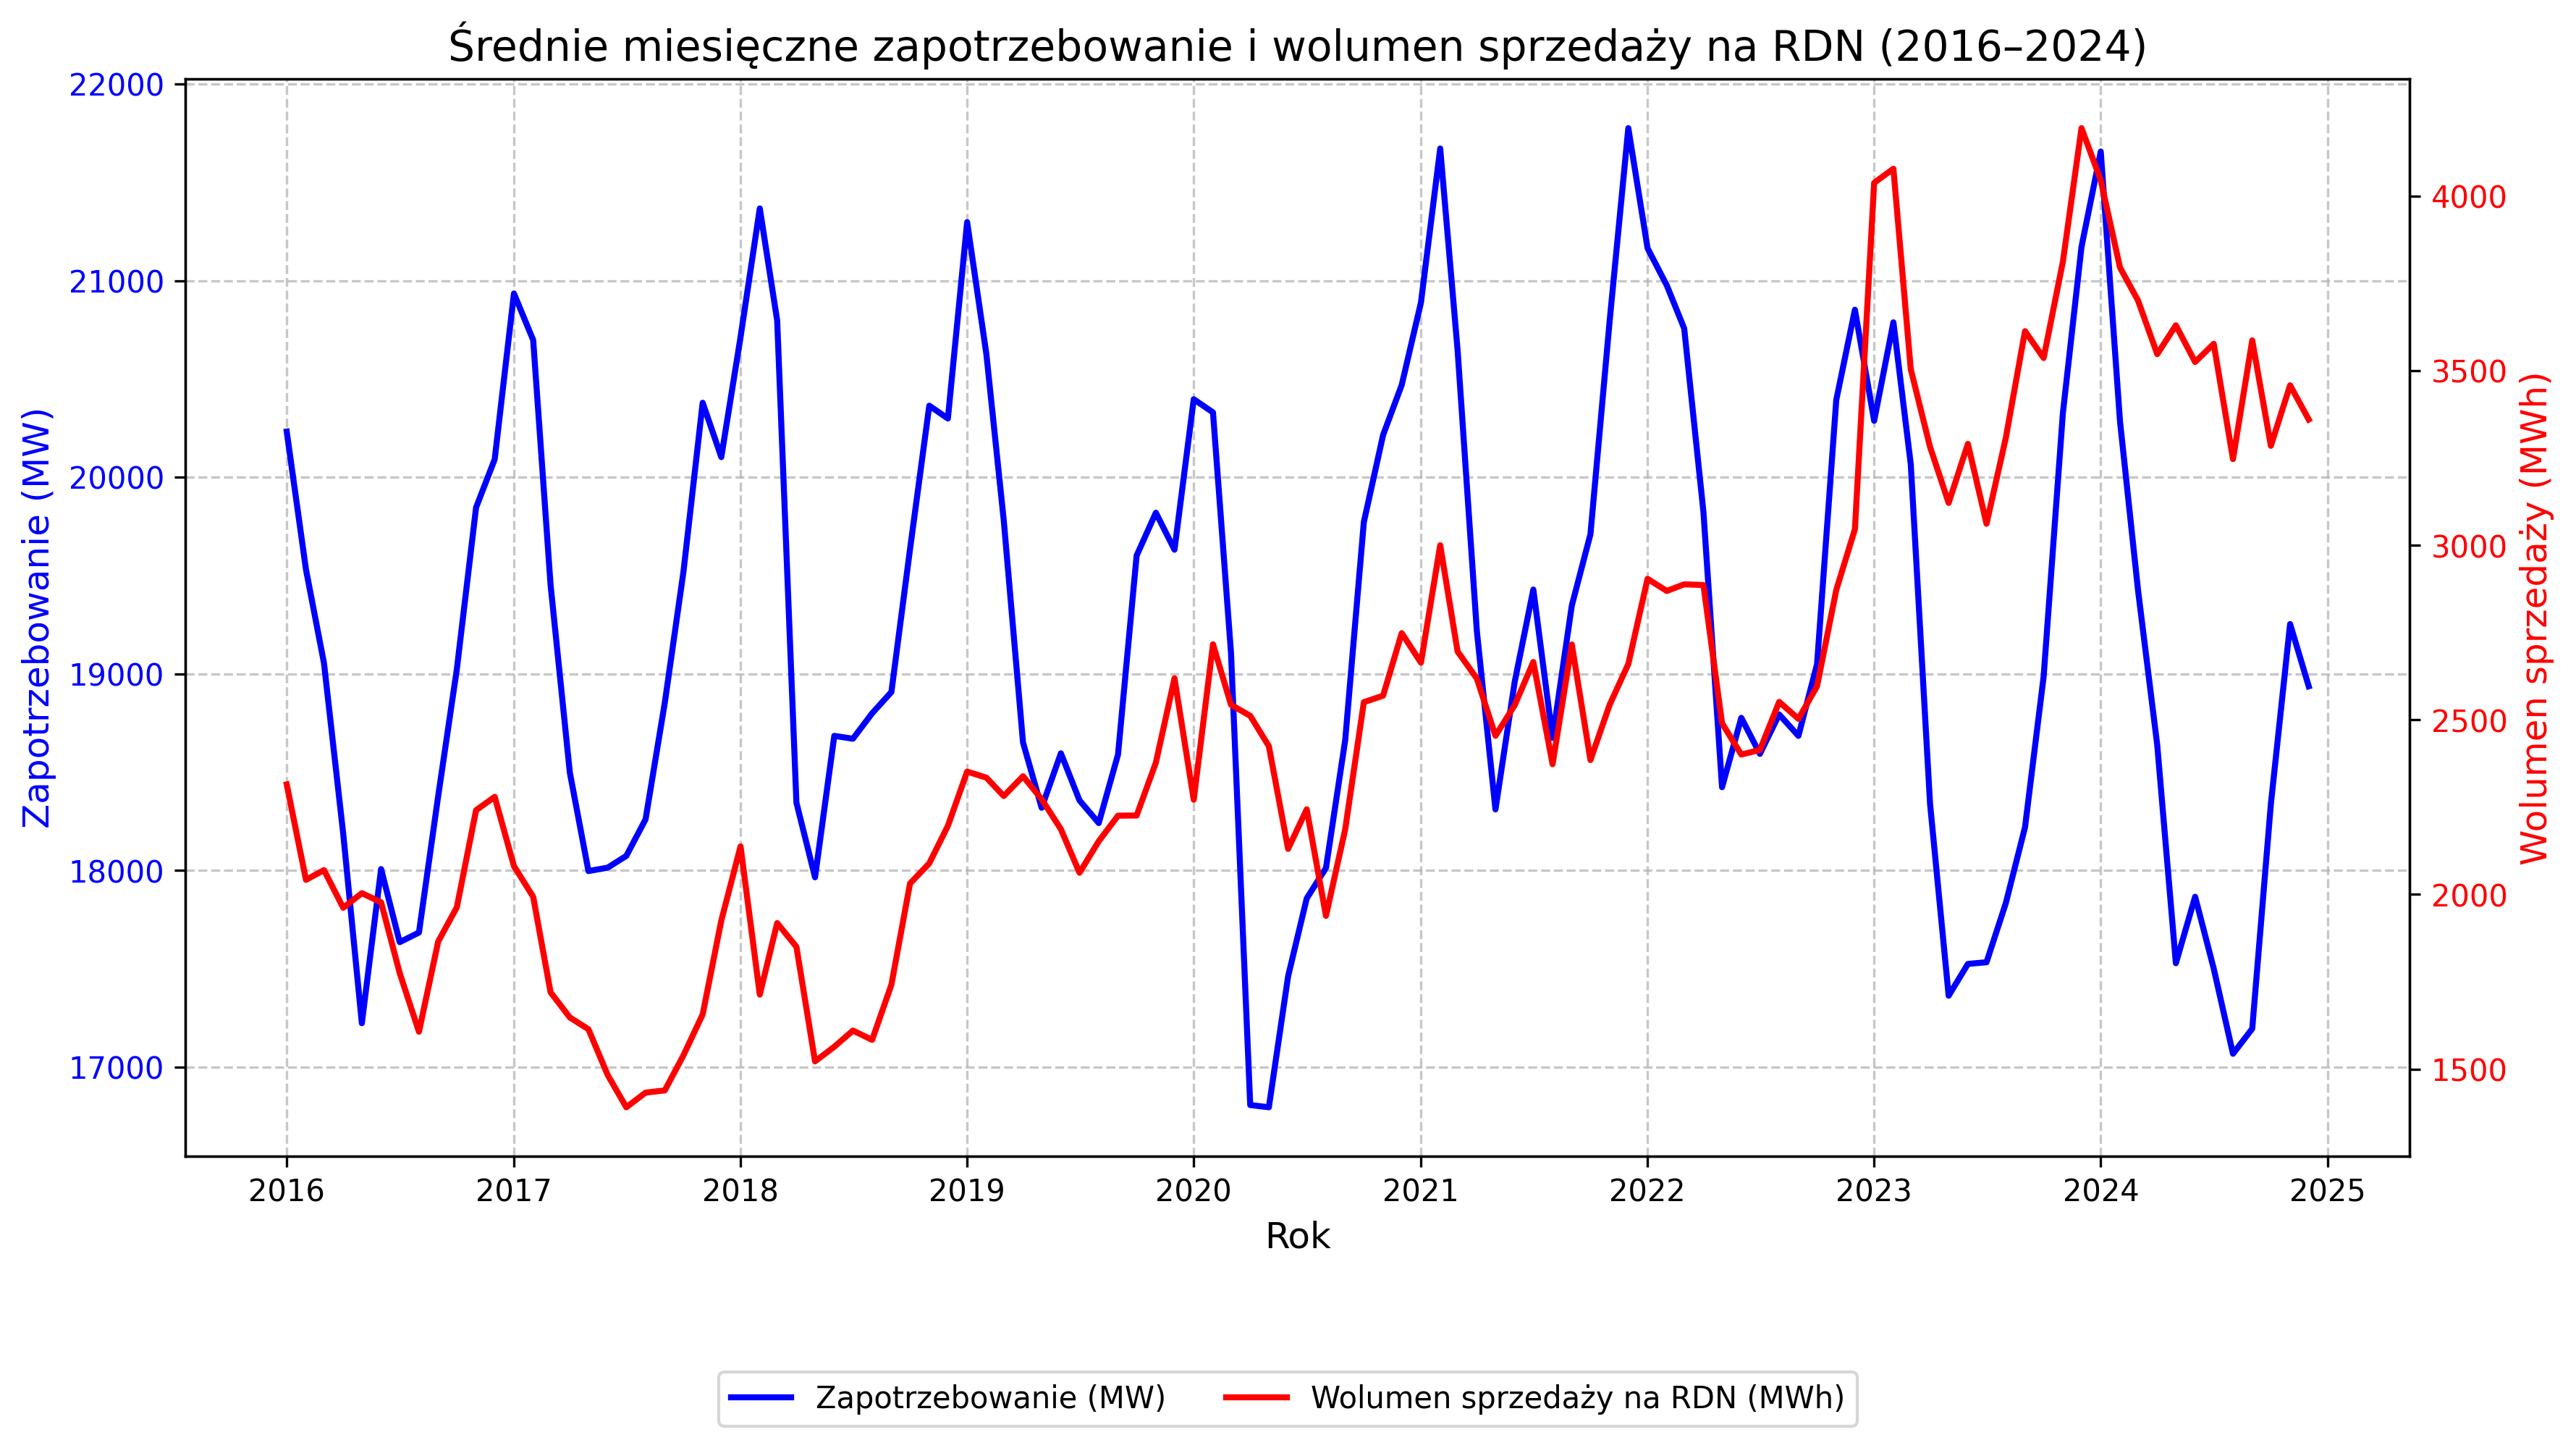
\includegraphics[width=0.9\textwidth]{../plots/market/load_vs_volume_2016_2024.png}
    \caption{Zapotrzebowanie na energię i wolumen handlu w latach 2016-2024 (w ujęciu miesięcznym). Źródło: Opracowanie własne na podstawie danych z PSE.}
    \label{fig:load_vs_trade_volume}
\end{figure}

Rozbieżność między zapotrzebowaniem a wolumenem sprzedaży na RDN ma swój powód. Wolumen sprzedaży na RDN zwykle nie przekracza 5000 MWh w porównaniu do zapotrzebowania na poziomie ponad 15 000  MWh wskazuje, że RDN pokrywa jedynie część \% całkowitego zapotrzebowania. Pozostała część jest zaspokajana przez: (1) kontrakty bilateralne (OTC), (2) rynek bilansujący, na którym PSE kupuje energię w czasie rzeczywistym, (3) import energii z sąsiednich krajów, jak pokazano w podrozdziale~\ref{subsec:trade} oraz innego rodzaju transakcje. 

Wyraźnie widoczne są duże szczyty zapotrzebowania zapotrzebowania w okresie zimowym. Wynika to z zwiększonego zapotrzebowania na energię elektryczną w okresie grzewczym, co jest typowe dla klimatu Polski.

\subsection{Inne zmienne}
\label{subsec:seasonal}

W swoim zbiorze danych uwzględnione zostały inne zmienne, które mogą mieć wpływ na ceny energii na RDN.

\subsubsection{Zmienne sezonowe}
\label{subsubsec:seasonal_variables}
Zmienne sezonowe, takie jak \texttt{day\_of\_week}, \texttt{month} i \texttt{is\_holiday}, zostały wprowadzone do zbioru danych w celu uchwycenia cykliczności i wzorców sezonowych w cenach energii na Rynku Dnia Następnego. Zmienne te zostały wygenerowane na podstawie kolumny \texttt{timestamp}, co pozwoliło na ich integrację z pozostałymi danymi w formacie godzinowym.

Zmienna \texttt{month} reprezentuje miesiąc roku (1-12, gdzie 1 to styczeń, a 12 to grudzień). Na temat cykliczności miesięcznej wspominałęm wcześniej w podrozdziałach \ref{subsec:prices} i \ref{subsec:demand}. Niemniej jednak, wprowadzenie zmiennych \texttt{day\_of\_week} i \texttt{month} do modelu pozwala lepiej uchwycić cykliczność i sezonowość w cenach energii, na poszczególne godziny dnia o czym świadczy poniższy wykres korelacji.

\begin{figure}[H]
    \centering
    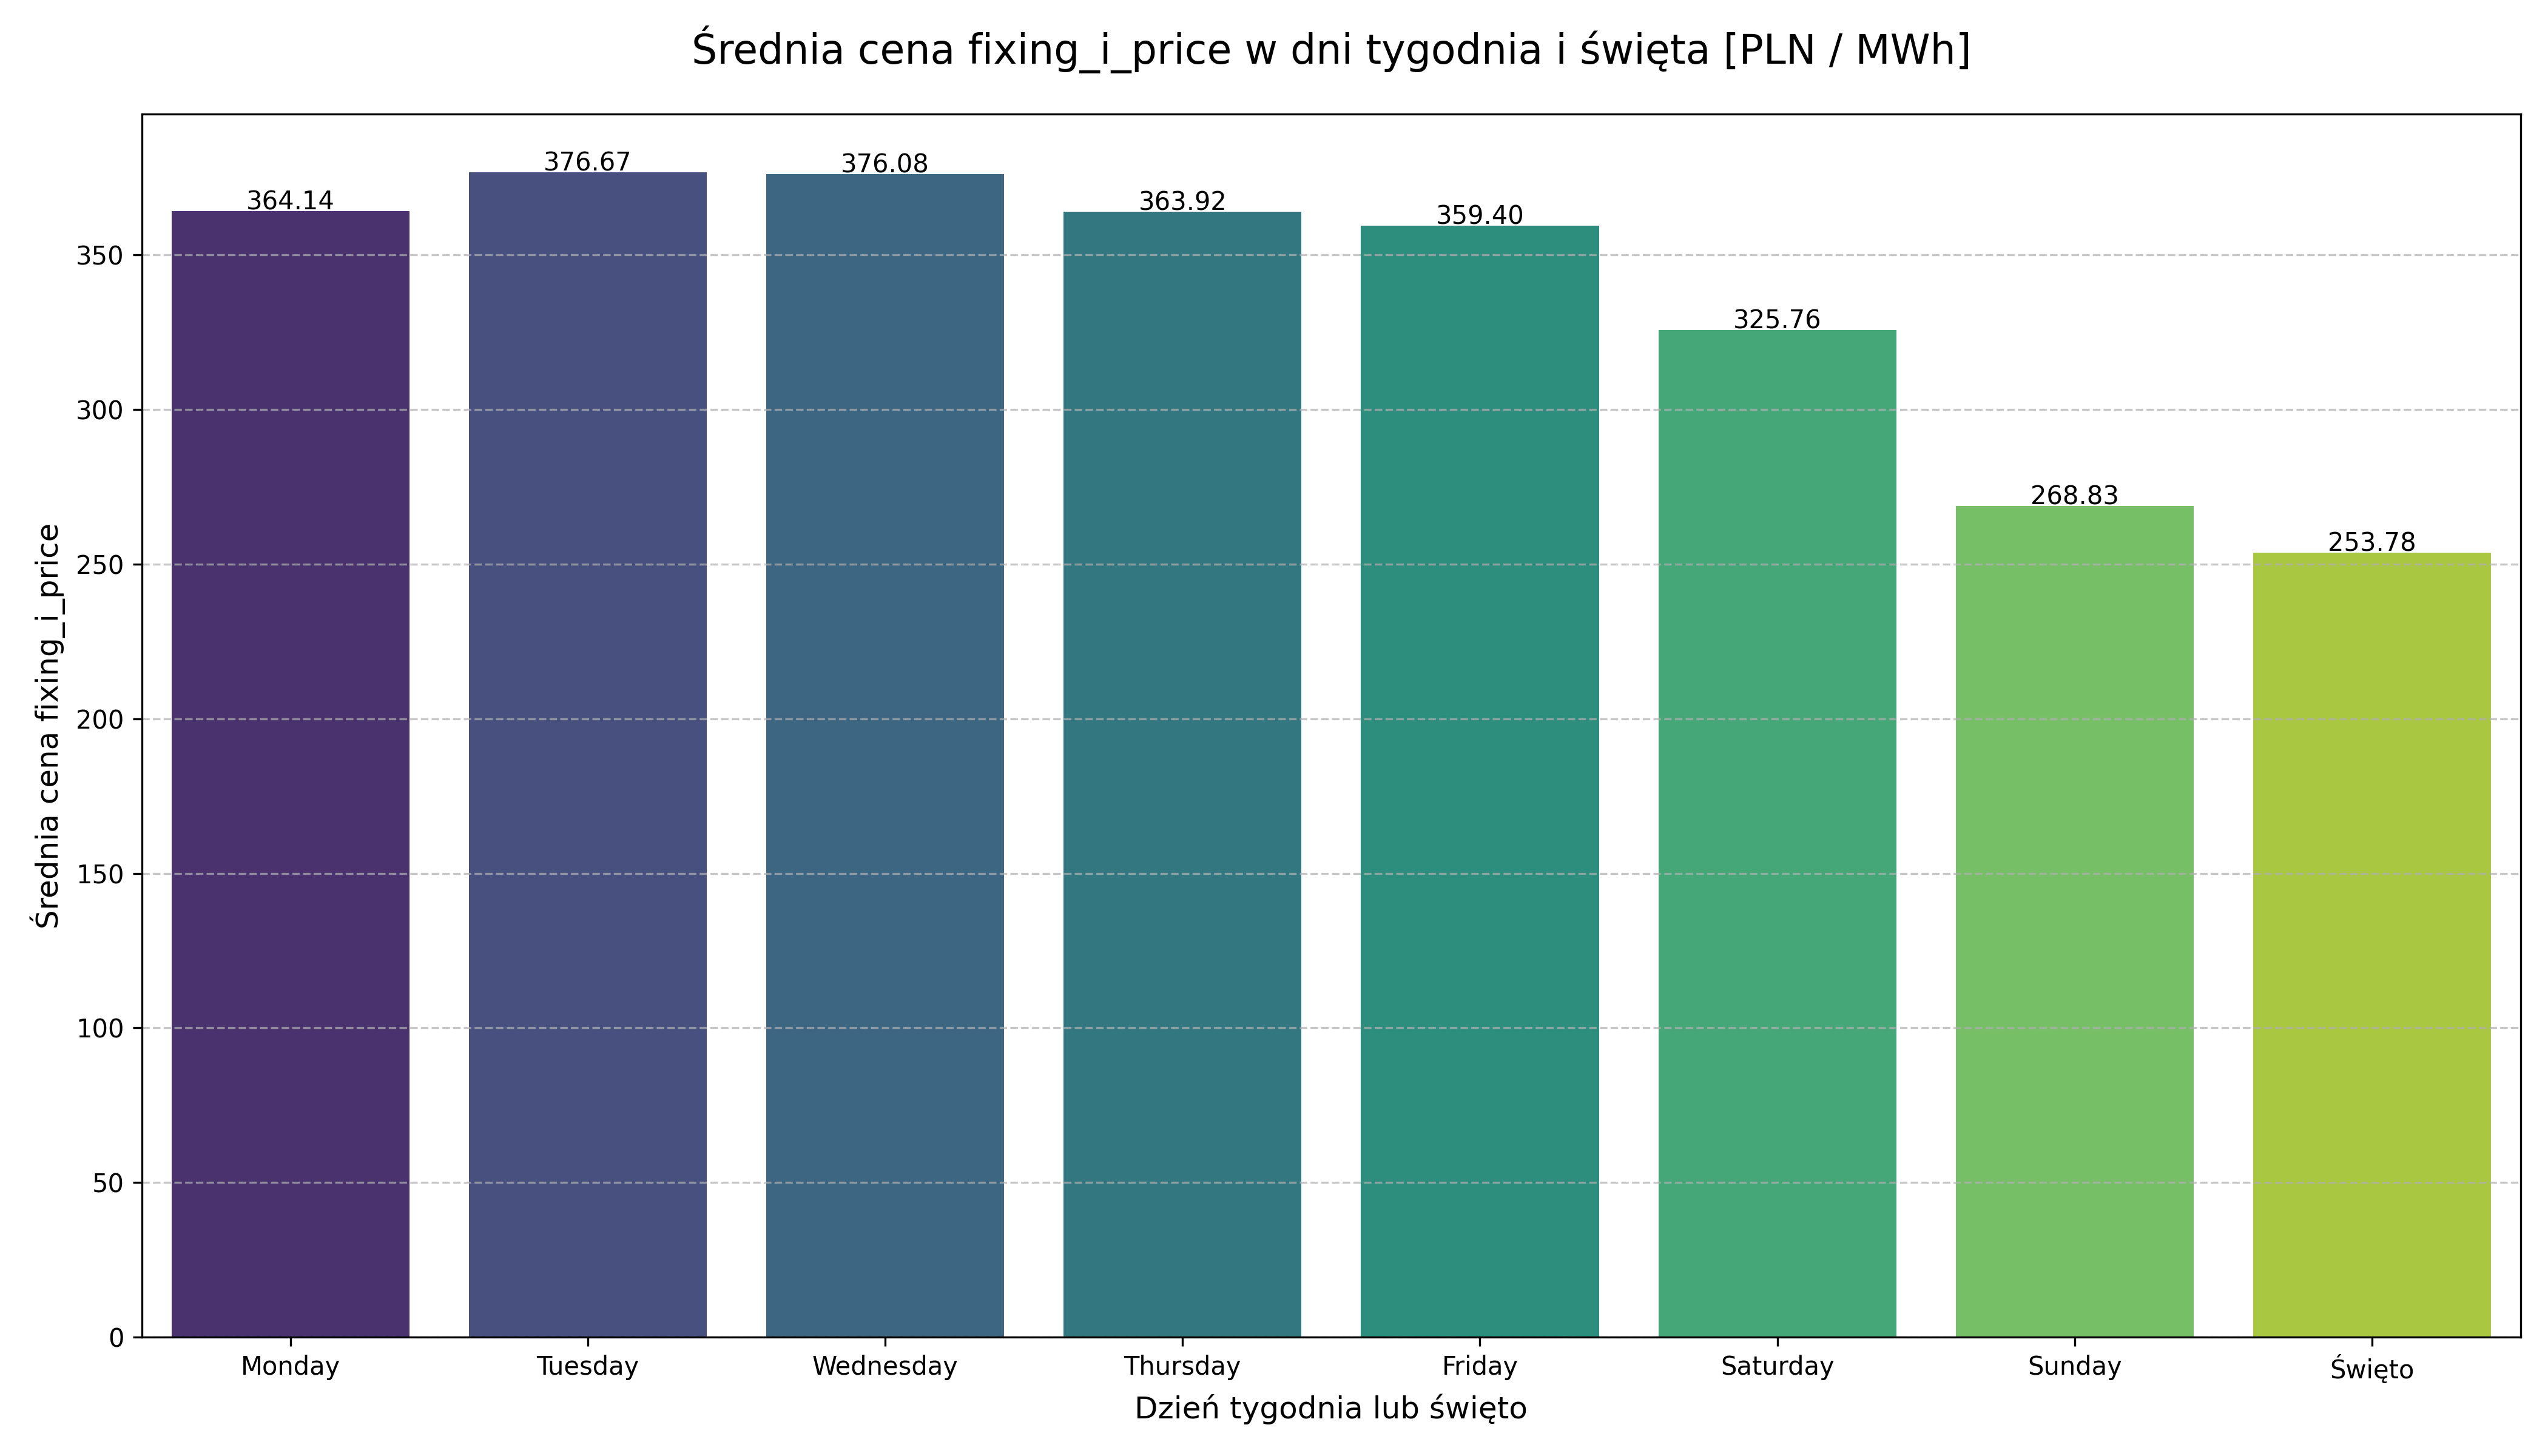
\includegraphics[width=0.9\textwidth]{../plots/fixing_i_price_weekdays_holidays.png}
    \caption{Korelacja dni tygodnia z cenami energii na RDN.}
    \label{fig:seasonal-correlation}
\end{figure}

Zmienna \texttt{day\_of\_week} reprezentuje dzień tygodnia (0-6, gdzie 0 to poniedziałek, a 6 to niedziela) i pozwala modelowi uwzględnić cykliczność tygodniową w cenach energii. Z wykresu wynika, że zapotrzebowanie na energię jest zazwyczaj wyższe w dni robocze, gdy działa przemysł i biura, a niższe w weekendy i święta, gdy aktywność gospodarcza jest mniejsza. Ta cykliczność przekłada się na ceny energii na RDN: w dni robocze ceny są zazwyczaj wyższe, szczególnie w godzinach szczytu. Wprowadzone zmienne sezonowe pozwalają modelowi lepiej uchwycić te wzorce, co jest istotne w zadaniu modelowania.

Dodatkowo wprowadzono zmienną \texttt{peak\_hour}, która jest zmienną binarną określającą godziny szczytu, w których występuje zwiększone zapotrzebowanie na energię elektryczną. Przyjmuje wartość 1, jeśli spełniony jest jeden z dwóch warunków, w przeciwnym razie 0:
\begin{itemize}
    \item W dni wolne lub dni weekendowe, zapotrzebowanie przekracza 18 000 MW, a godzina należy do przedziałów porannych (7:00-9:00) lub wieczornych (16:00-18:00).
    \item W dni robocze, zapotrzebowanie przekracza 23 000 MW i posiada takie same przedziały godzinowe jak w dni wolne.
\end{itemize}
Definicja ta odzwierciedla wyższe zapotrzebowanie na energię w godzinach szczytu, z różnymi progami dla dni roboczych i wolnych, co jest zgodne z charakterystyką polskiego rynku energii.

\subsubsection{Ceny historyczne}
\label{subsec:historical_prices}
 
Zmienne historyczne \texttt{fixing\_i\_price\_lag24}, \texttt{fixing\_i\_price\_lag48}, \texttt{fixing\_i\_price\_lag72}, \texttt{fixing\_i\_price\_lag96}, \texttt{fixing\_i\_price\_lag120}, \texttt{fixing\_i\_price\_lag144} oraz \newline \texttt{fixing\_i\_price\_lag168}, zostały wprowadzone do zbioru danych w celu uchwycenia autokorelacji w cenach energii na RDN. Zmienne te zostały wygenerowane na podstawie kolumny \texttt{fixing\_i\_price}, która reprezentuje cenę energii na RDN w danej godzinie (w PLN/MWh), poprzez przesunięcie wartości o odpowiednią liczbę godzin. 

Opróćz ceny opóźnionej, zostały wprowadzone średnie kroczące z ostatnich 24 i 48 godzin. W wyniku tego do datasetu zostały dodane zmienne \texttt{fixing\_i\_price\_mean24} i \texttt{fixing\_i\_price\_mean48}, które reprezentują średnie ceny energii na RDN w ostatnich 24 i 48 godzinach. Wartości te zostały obliczone na podstawie danych z kolumny \texttt{fixing\_i\_price} z przesunięciem o jedną godzinę, żeby nie w średniej kroczącej nie brać pod uwagę obecnej wartości. 

Wprowadzenie zmiennych historycznych do modelu pozwala lepiej uchwycić autokorelację i cykliczność w cenach energii, co jest kluczowe dla poprawy dokładności prognoz. Zgodnie z literaturą, ceny historyczne są często jednymi z najważniejszych predyktorów w modelach prognozowania cen energii, szczególnie w modelach autoregresyjnych i modelach uczenia maszynowego.

\subsubsection{Kurs wymiany PLN/USD}
\label{subsec:pln_usd}

Zmienna \texttt{pln\_usd} reprezentuje kurs wymiany złotego polskiego względem dolara amerykańskiego (USD/PLN) w danej godzinie. Dane te zostały pozyskane z oficjalnej strony Narodowego Banku Polskiego (NBP) w granulacji dziennej. W celu dopasowania danych do godzinowego formatu RDN, wartości kursu zostały przypisane do wszystkich godzin w danym dniu. W przypadku dni wolnych od pracy lub braku dostępnych danych, wartości kursu zostały interpolowane.

\begin{table}[H]
    \centering
    \begin{tabular}{|c|c|}
    \hline
    \textbf{Rok} & \textbf{Średni kurs PLN/USD} \\ \hline
    2016 & 3.94 \\ \hline
    2017 & 3.78 \\ \hline
    2018 & 3.61 \\ \hline
    2019 & 3.84 \\ \hline
    2020 & 3.90 \\ \hline
    2021 & 3.86 \\ \hline
    2022 & 4.46 \\ \hline
    2023 & 4.20 \\ \hline
    2024 & 3.98 \\ \hline
    \end{tabular}
    \caption{Średni kurs wymiany PLN/USD w latach 2016-2024. Źródło: Opracowanie własne na podstawie danych NBP.}
    \label{tab:pln-usd-exchange-rate}
\end{table}

Kurs wymiany PLN/USD jest istotnym czynnikiem w kontekście prognozowania cen energii na RDN, ponieważ Polska importuje znaczną część paliw kopalnych, takich jak gaz ziemny i ropa naftowa, które są wyceniane w dolarach amerykańskich. Wzrost kursu PLN/USD (czyli osłabienie złotego względem dolara) zwiększa koszty importu tych paliw. Kurs polskiego złotego odzwierciedla też zmiany w gospodarce krajowej i globalnej. Próbując stabilizować kurs złotego, NBP zmienia politykę monetarną kraju, co może wpływać na ceny energii.